\documentclass[12pt,a4paper]{article}

% ------------------------------------------------------------------
% Compilation note:
% This English version is intended to be compiled with XeLaTeX.
% Figures must be available in docs/experiments/figures/.
% Figure1.png and Figure2.png describe the MV-DUSt3R+ architecture/pipeline.
% Depth-estimator fine-tuning plots are stored in docs/experiments/figures/.
% ------------------------------------------------------------------

\usepackage[margin=1in]{geometry}
\usepackage{fontspec}
\IfFontExistsTF{Times New Roman}{\setmainfont{Times New Roman}}{\setmainfont{TeX Gyre Termes}}
\usepackage{setspace}
\usepackage{titlesec}
\usepackage{tocloft}
\usepackage{array}
\usepackage{booktabs}
\usepackage{longtable}
\usepackage{multirow}
\usepackage{graphicx}
\graphicspath{{figures/}}
\usepackage{float}
\usepackage{amsmath,amssymb}
\usepackage{caption}
\usepackage{subcaption}
\usepackage{enumitem}
\usepackage{xcolor}
\usepackage{tikz}
\usetikzlibrary{arrows.meta,positioning,fit,calc,shapes.geometric}
\usepackage[hidelinks]{hyperref}
\usepackage{url}

\setstretch{1.15}
\setlength{\parindent}{0.45in}
\setlength{\parskip}{0pt}
\titleformat{\section}{\normalfont\Large\bfseries}{\thesection.}{0.5em}{}
\titleformat{\subsection}{\normalfont\large\bfseries}{\thesubsection}{0.5em}{}
\titleformat{\subsubsection}{\normalfont\normalsize\bfseries\itshape}{\thesubsubsection}{0.5em}{}
\captionsetup{font=small,labelfont=bf}
\renewcommand{\cftsecleader}{\cftdotfill{\cftdotsep}}

\newcommand{\ours}{Estimated-Depth Correction}
\newcommand{\mvd}{MV-DUSt3R}
\newcommand{\mvdp}{MV-DUSt3R+}
\newcommand{\da}{Depth Anything V2}

\begin{document}

% ------------------------------------------------------------------
% Title page
% ------------------------------------------------------------------
\begin{titlepage}
\centering
{\Large HANOI UNIVERSITY OF SCIENCE AND TECHNOLOGY\\}
\vspace{0.2cm}
{\large School of Information and Communication Technology\\}
\vspace{1.0cm}

\includegraphics[scale=0.13]{logo-soict-hust-1.png}\\
\vspace{1.0cm}
{\Large Computer Vision Project Report\\}
\vspace{1.2cm}
{\LARGE\bfseries Sparse-View RGB 3D Scene Reconstruction\\}
\vspace{0.2cm}
{\LARGE\bfseries A Diagnostic Study of Estimated-Depth Correction\\}
\vspace{2.0cm}
\begin{flushleft}
\hspace{2.8cm}\textbf{Students:}\\
\hspace{2.8cm}Nguyen Ngoc Minh - 20235533\\
\hspace{2.8cm}Kieu Son Tung - 20235571\\
\hspace{2.8cm}Dang Thinh Tuong Minh - 20235528\\
\vspace{0.3cm}
\hspace{2.8cm}\textbf{Supervisor:} Tran Nguyen Ngoc\\
\end{flushleft}
\vfill
{Hanoi, June 25, 2026}
\end{titlepage}

\pagenumbering{roman}
\tableofcontents
\newpage
\pagenumbering{arabic}

% ------------------------------------------------------------------
\section{Introduction}
Three-dimensional scene reconstruction is a fundamental problem in computer vision. It supports applications such as augmented reality, robotics, digital twins, indoor mapping, visual localization, and 3D content creation. Classical reconstruction pipelines usually require many images, calibrated cameras, reliable pose estimation, feature matching, structure-from-motion, and multi-view stereo. Although these systems can produce high-quality geometry, they are difficult to deploy when only a small number of ordinary RGB images are available.

In practical settings, the input is often sparse. A user may only have three to five images of an indoor scene, captured by a standard phone camera. These images usually contain RGB appearance only. They do not provide measured depth maps, camera intrinsics, or camera poses. 

Recent feed-forward reconstruction models such as \mvdp{} reduce this dependency by reconstructing 3D scenes from multiple unposed RGB views. \mvdp{} is designed for sparse multi-view RGB input and directly predicts pixel-aligned 3D pointmaps without requiring camera poses or depth maps during inference. The official project describes \mvdp{} as a model that reconstructs large scenes from multiple unposed RGB views \cite{mvdust3r_project,mvdust3r_paper}. This makes \mvdp{} a highly capable backbone for sparse-view RGB-only reconstruction.

However, relying strictly on RGB appearance for full 3D geometry remains difficult. Appearance alone is often insufficient for metric depth recovery in low-texture areas, occluded regions, repeated structures, and low-overlap views. Monocular depth estimation is also inherently ambiguous because a single image loses metric scale under perspective projection. Therefore, while an RGB-only backbone can generate visually plausible structures, the resulting candidate points are often geometrically misaligned, distorted, or completely folded in ambiguous regions.

To study this problem, this project investigates an RGB-only reconstruction pipeline assisted by estimated depth. Instead of treating \mvdp{} only as a final point-cloud generator, the pipeline uses it as a strong RGB-only multi-view backbone and studies whether monocular estimated depth can serve as an additional geometric prior for correction. The depth maps are produced by a fine-tuned monocular depth estimator, while the correction stage tests how reliably these estimated-depth anchors can be fused with \mvdp{} candidate geometry.

The main motivation is practical deployment. The system should require only sparse RGB views at deployment time, satisfying the RGB-only contract. The fine-tuned depth estimator provides useful per-pixel geometric priors, but the completed reconstruction experiments show that the current fusion and correction rule is the main bottleneck. In particular, fine-tuned estimated-depth correction does not outperform the RGB-only \mvdp{} baseline in the reported table.

The main contributions of this report are:
\begin{enumerate}[leftmargin=1.2cm]
    \item It studies a diagnostic pipeline that combines the RGB-only \mvdp{} backbone with a fine-tuned monocular depth estimator.
    \item It implements an estimated-depth correction module to test whether predicted metric depth can be fused reliably with candidate multi-view geometry.
    \item It defines a sparse-view RGB-only reconstruction setting in which measured depth is used only for training and evaluation.
    \item It reports both depth-estimation quality and 3D point-cloud reconstruction metrics, showing that fine-tuned depth is a useful prior but current correction is not yet strong enough to beat \mvdp{}.
\end{enumerate}

% ------------------------------------------------------------------
\section{Background and Related Work}
This section reviews three related directions: sparse-view RGB-only reconstruction, monocular depth estimation, and depth-assisted 3D reconstruction. These areas motivate the diagnostic pipeline studied in this report.

\subsection{Sparse-View RGB-Only 3D Reconstruction}
Traditional multi-view reconstruction is usually implemented as a multi-stage pipeline consisting of feature detection, feature matching, camera pose estimation, triangulation, bundle adjustment, and dense multi-view stereo. This modular design is interpretable and has been validated in many practical systems. However, each stage depends on the quality of previous stages, so errors can accumulate. These systems also typically require sufficient view overlap, reliable intrinsics, and accurate camera poses.

Recent learning-based methods move toward direct reconstruction from unposed RGB images. DUSt3R predicts 3D pointmaps from pairs of RGB images without known camera intrinsics or poses, and MASt3R extends this direction with dense matching grounded in 3D representations \cite{dust3r_paper,mast3r_paper}. When more than two images are used, pairwise methods must construct many local reconstructions and then align them through global optimization. The \mvdp{} paper notes that pairwise reconstructions may contain matching or geometric errors, and that global optimization cannot always remove these errors \cite{mvdust3r_paper}.

\mvd{} handles multiple views in a single feed-forward pass. Instead of exchanging information only between two images, it uses multi-view decoder blocks so that each view can receive information from all other views. \mvdp{} further improves stability by using multiple reference views and cross-reference-view blocks, allowing the model to fuse information across different reference choices \cite{mvdust3r_paper}.

In this project, \mvdp{} is used as the RGB-only multi-view reconstruction backbone. It produces the initial point cloud from a small number of input images. The RGB-only reconstruction is treated as candidate geometry, which can then be checked and corrected using estimated depth.

\subsection{Monocular Depth Estimation}
Monocular depth estimation predicts a dense depth map from a single RGB image. It is attractive for practical applications because it does not require stereo images or depth sensors. However, the problem is ill-posed. A single image cannot fully determine metric scale because different 3D scenes may project to similar 2D images. Recent work on scale ambiguity in monocular depth also emphasizes that metric depth from one image is under-constrained by perspective projection \cite{rsa_depth}.

Large-scale depth models such as \da{} improve monocular depth estimation through strong pretrained encoders and large training corpora. \da{} provides robust depth predictions and includes metric-depth variants obtained by fine-tuning pretrained encoders with metric depth labels \cite{depthanything_project,depthanything_metric}. This makes it a suitable initialization for the project. The fine-tuning stage uses RGB-D data as supervision so that the depth estimator adapts to indoor scenes and the reconstruction evaluation protocol.

\subsection{Depth-Assisted 3D Reconstruction}
Depth maps provide strong geometric information for 3D reconstruction. If measured depth and camera poses are available, a point cloud can be constructed by back-projecting valid depth pixels into 3D. However, this assumes that the user has a depth sensor and camera geometry at inference time. This assumption conflicts with the RGB-only deployment goal.

An intermediate solution is to use predicted depth instead of measured depth. Predicted depth is imperfect, but it can still provide useful geometric priors. In this project, predicted depth does not replace the multi-view backbone. Instead, it is used as a correction signal for candidate geometry. This design keeps the multi-view reasoning of \mvdp{} while using learned depth priors to reduce wrong-depth errors.

\subsection{Project Positioning}
This project does not train a new reconstruction backbone from scratch. Instead, it builds a structured diagnostic pipeline on top of modern components. \mvdp{} provides candidate geometry from sparse RGB views, while the fine-tuned depth estimator provides a per-image metric-depth prior. The main contribution is the experimental setting, the depth fine-tuning process, and the analysis of the correction bottleneck: using RGB-D data during development while keeping the final inference contract RGB-only.

% ------------------------------------------------------------------
\section{Model Architectures Used in the Project}
This section describes the two main model components used in the pipeline: \mvdp{} and \da{} Metric Indoor. It is placed before the dataset section so that the reader can understand what each model receives, what it outputs, and how it contributes to the final system.

\subsection{MV-DUSt3R+ Backbone}
\mvdp{} is a feed-forward sparse-view scene reconstruction model. Its input is a set of RGB images. Its output is a set of pixel-aligned 3D pointmaps and associated confidence information. Compared with pairwise DUSt3R-style reconstruction, \mvdp{} is designed to reason over multiple input views in one stage. It uses cross-reference-view reasoning to reduce sensitivity to the selected reference view and to improve stability in sparse-view settings.

In this project, \mvdp{} is used only as a frozen or pretrained reconstruction backbone. The project does not claim to modify the \mvdp{} architecture. Instead, \mvdp{} produces the RGB-only candidate point cloud. The estimated-depth branch is then evaluated as a diagnostic correction signal for this candidate point cloud.

\begin{figure}[H]
    \centering
    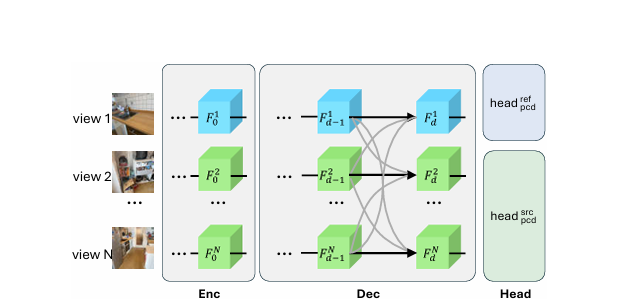
\includegraphics[width=0.95\linewidth]{Figure1.png}
    \caption{High-level \mvdp{} sparse-view reconstruction architecture used as the RGB-only backbone, adapted from Tang et al.~\cite{mvdust3r_paper}.}
    \label{fig:mvd_arch}
\end{figure}

\begin{figure}[H]
    \centering
    
\includegraphics[width=0.95\linewidth]{mv_overview.png}
    \caption{Detailed overview of the \mvdp{} cross-view reasoning process, adapted from Tang et al.~\cite{mvdust3r_paper}.}
    \label{fig:mvd_overview}
\end{figure}

\subsection{Depth Anything V2 Metric Indoor}
The depth estimator is initialized from \da{} Metric Indoor. This model predicts a dense metric depth map from a single RGB image. The pretrained checkpoint already provides useful indoor depth priors, but the project fine-tunes it on the available RGB-D data so that it better matches the dataset distribution and the reconstruction pipeline.

At inference time, the depth estimator receives each sparse RGB input view independently and predicts an estimated depth map. These estimated depth maps are then used as source-depth anchors for point-cloud correction. Because the depth is predicted from RGB, the evaluated pipeline still satisfies the RGB-only input contract.


% ------------------------------------------------------------------
\section{Problem Formulation}
Let a sparse group contain \(N\) RGB views:
\[
\mathcal{I}=\{I_1,I_2,\ldots,I_N\}, \quad N\in\{3,4,5\}.
\]
The final inference-time input is only the RGB images. During development, the dataset also provides measured depth maps and camera information that can be used for supervision and evaluation:
\[
\mathcal{D}^{\mathrm{gt}}=\{D^{\mathrm{gt}}_1,D^{\mathrm{gt}}_2,\ldots,D^{\mathrm{gt}}_N\}, \quad
\mathcal{K}^{\mathrm{gt}}=\{K^{\mathrm{gt}}_1,K^{\mathrm{gt}}_2,\ldots,K^{\mathrm{gt}}_N\}, \quad
\mathcal{T}^{\mathrm{gt}}=\{T^{\mathrm{gt}}_1,T^{\mathrm{gt}}_2,\ldots,T^{\mathrm{gt}}_N\}.
\]
The measured depth maps \(\mathcal{D}^{\mathrm{gt}}\), measured intrinsics \(\mathcal{K}^{\mathrm{gt}}\), and measured camera poses \(\mathcal{T}^{\mathrm{gt}}\) are not final deployment inputs. They are used to supervise the depth estimator, to build reference geometry, and to evaluate reconstruction quality.

The \mvdp{} backbone predicts candidate points and an internal camera geometry estimate:
\[
P_{\mathrm{mv}}, \hat{\mathcal{K}}, \hat{\mathcal{T}}, C_{\mathrm{mv}}
= f_{\mathrm{mv}}(\mathcal{I}).
\]
Here, \(P_{\mathrm{mv}}\) is the candidate point cloud, \(\hat{\mathcal{K}}\) denotes the estimated intrinsics, \(\hat{\mathcal{T}}\) denotes the estimated camera-to-world poses, and \(C_{\mathrm{mv}}\) denotes the model confidence. This notation is important because the RGB-only setting cannot rely on externally provided camera calibration at inference time.

The fine-tuned depth estimator predicts depth maps from RGB:
\[
\hat{D}_i = f_{\mathrm{depth}}(I_i).
\]
Let \(\hat{\mathcal{D}}_{\mathrm{est}}=\{\hat{D}_1,\hat{D}_2,\ldots,\hat{D}_N\}\) denote the full set of estimated depth maps for the sparse group.
The correction module under study produces the final point cloud:
\[
P_{\mathrm{corr}} = C(P_{\mathrm{mv}}, \hat{\mathcal{D}}_{\mathrm{est}}, \hat{\mathcal{K}}, \hat{\mathcal{T}}).
\]
Thus, the intended deployment contract is:
\[
\{I_1,\ldots,I_N\}
\longrightarrow
\{P_{\mathrm{mv}},\hat{\mathcal{K}},\hat{\mathcal{T}},\hat{\mathcal{D}}_{\mathrm{est}}\}
\longrightarrow
P_{\mathrm{corr}}.
\]
Here, \(\hat{\mathcal{D}}_{\mathrm{est}}\) denotes the estimated depth maps produced from RGB images, not the measured depth maps from the dataset.
Measured RGB-D information remains a training and evaluation resource, not an inference-time requirement.

% ------------------------------------------------------------------
\section{Diagnostic Estimated-Depth Correction}
\subsection{Pipeline Overview}
The diagnostic pipeline has three stages:
\begin{enumerate}[leftmargin=1.2cm]
    \item \textbf{RGB-only candidate reconstruction.} Sparse RGB views are passed into \mvdp{} to obtain candidate 3D points and confidence scores.
    \item \textbf{Monocular estimated depth.} Each input RGB image is passed through the fine-tuned \da{} Metric Indoor estimator to predict a depth map.
    \item \textbf{Estimated-depth correction.} Candidate points are compared with points back-projected from estimated depth. Points with large residuals are moved toward the estimated-depth anchor.
\end{enumerate}

This design is intentionally conservative. It does not replace multi-view reconstruction with monocular depth alone. Instead, depth is used as a correction signal for the multi-view candidate geometry.

\subsection{Independent Feature Extraction}
Before applying correction, the two geometric cues are extracted independently. The \mvdp{} branch processes the whole sparse RGB group jointly:
\[
P_{\mathrm{mv}}, \hat{K}_i, \hat{T}_i, c^{\mathrm{mv}}_i
= f_{\mathrm{mv}}(I_1,\ldots,I_N),
\]
where \(P_{\mathrm{mv}}\) is the candidate multi-view geometry, \(\hat{K}_i\) is the estimated intrinsic matrix for view \(i\), \(\hat{T}_i\) is the estimated camera-to-world transform, and \(c^{\mathrm{mv}}_i\) is the confidence associated with the \mvdp{} prediction.

In parallel, the monocular depth branch processes each RGB image independently:
\[
\hat{D}_i = f_{\mathrm{depth}}(I_i),
\]
where \(\hat{D}_i(u,v)\) is the estimated metric depth value at pixel \((u,v)\). The intuition is that \mvdp{} contributes global multi-view structure and relative camera geometry, while the fine-tuned depth estimator contributes a per-pixel metric-depth prior. The correction stage is the only place where these two branches are fused.

\subsection{Back-Projection from Estimated Depth}
For a source pixel \((u,v)\) in view \(i\), the estimated depth is \(\hat{z}=\hat{D}_i(u,v)\). In the final RGB-only setting, \(\hat{K}_i\) and \(\hat{T}_i\) denote the camera intrinsics and camera-to-world pose estimated by the \mvdp{} branch. The corresponding point in camera coordinates is:
\begin{equation}
\hat{X}^{\mathrm{cam}}_{\mathrm{src}}(u,v) =
\hat{z}\hat{K}_i^{-1}
\begin{bmatrix}
u\\v\\1
\end{bmatrix}.
\end{equation}
Assuming \(\hat{T}_i\in\mathbb{R}^{4\times4}\) is a homogeneous camera-to-world transform, the world-coordinate point is:
\begin{equation}
\begin{bmatrix}
\hat{X}^{\mathrm{world}}_{\mathrm{src}}(u,v)\\
1
\end{bmatrix}
=
\hat{T}_i
\begin{bmatrix}
\hat{X}^{\mathrm{cam}}_{\mathrm{src}}(u,v)\\
1
\end{bmatrix}.
\end{equation}

\subsection{Residual-Gated Correction}
Let \(X_{\mathrm{pred}}(u,v)\) be the \mvdp{} candidate point associated with the same source pixel. The residual between candidate geometry and estimated-depth geometry is:
\begin{equation}
r(u,v)=\left\|X_{\mathrm{pred}}(u,v)-\hat{X}^{\mathrm{world}}_{\mathrm{src}}(u,v)\right\|_2.
\end{equation}
The corrected point is:
\begin{equation}
X_{\mathrm{corr}}(u,v)=
\begin{cases}
(1-\alpha)X_{\mathrm{pred}}(u,v)+\alpha\hat{X}^{\mathrm{world}}_{\mathrm{src}}(u,v), & r(u,v)\geq\tau,\\
X_{\mathrm{pred}}(u,v), & r(u,v)<\tau.
\end{cases}
\end{equation}
Here, \(\tau\) is the correction threshold and \(\alpha\) is the correction weight. In the estimated-depth correction experiments, the selected policy uses \(\tau=0.50\,\mathrm{m}\) and \(\alpha=0.25\). The intended final setting uses estimated depth from the fine-tuned model, not measured RGB-D source depth.

% ------------------------------------------------------------------
\section{Dataset and Experimental Setting}

\subsection{Dataset Overview and Inputs}
The experiments are conducted using a controlled indoor dataset derived from ScanNet \cite{scannet}. ScanNet is a large-scale, richly-annotated RGB-D video dataset containing 2.5 million views across more than 1,500 indoor scans. The dataset was gathered using a mobile setup consisting of an iPad Air 2 paired with an Occipital Structure Sensor, which simultaneously captured both RGB imagery and active depth maps at 30 frames per second. 

The collected scans encompass a wide variety of typical indoor environments--such as offices, living rooms, bedrooms, and bathrooms--presenting significant structural complexities, including heavy furniture occlusion, textureless walls, and reflective surfaces. For each scene, the dataset provides aligned RGB and depth frames, globally optimized 6-DoF camera poses, and a dense reconstructed 3D mesh.

The dataset is used in two different roles. At training time, measured RGB-D frames provide supervision for the monocular depth estimator. At evaluation time, measured depth, camera geometry, and reconstructed 3D references are used to compute quantitative metrics. At deployment time, however, the reconstruction pipeline receives only the sparse RGB views. This separation is essential: the project is not a depth-sensor reconstruction system, but an RGB-only system trained and evaluated with RGB-D supervision.

\begin{figure}[H]
    \centering
    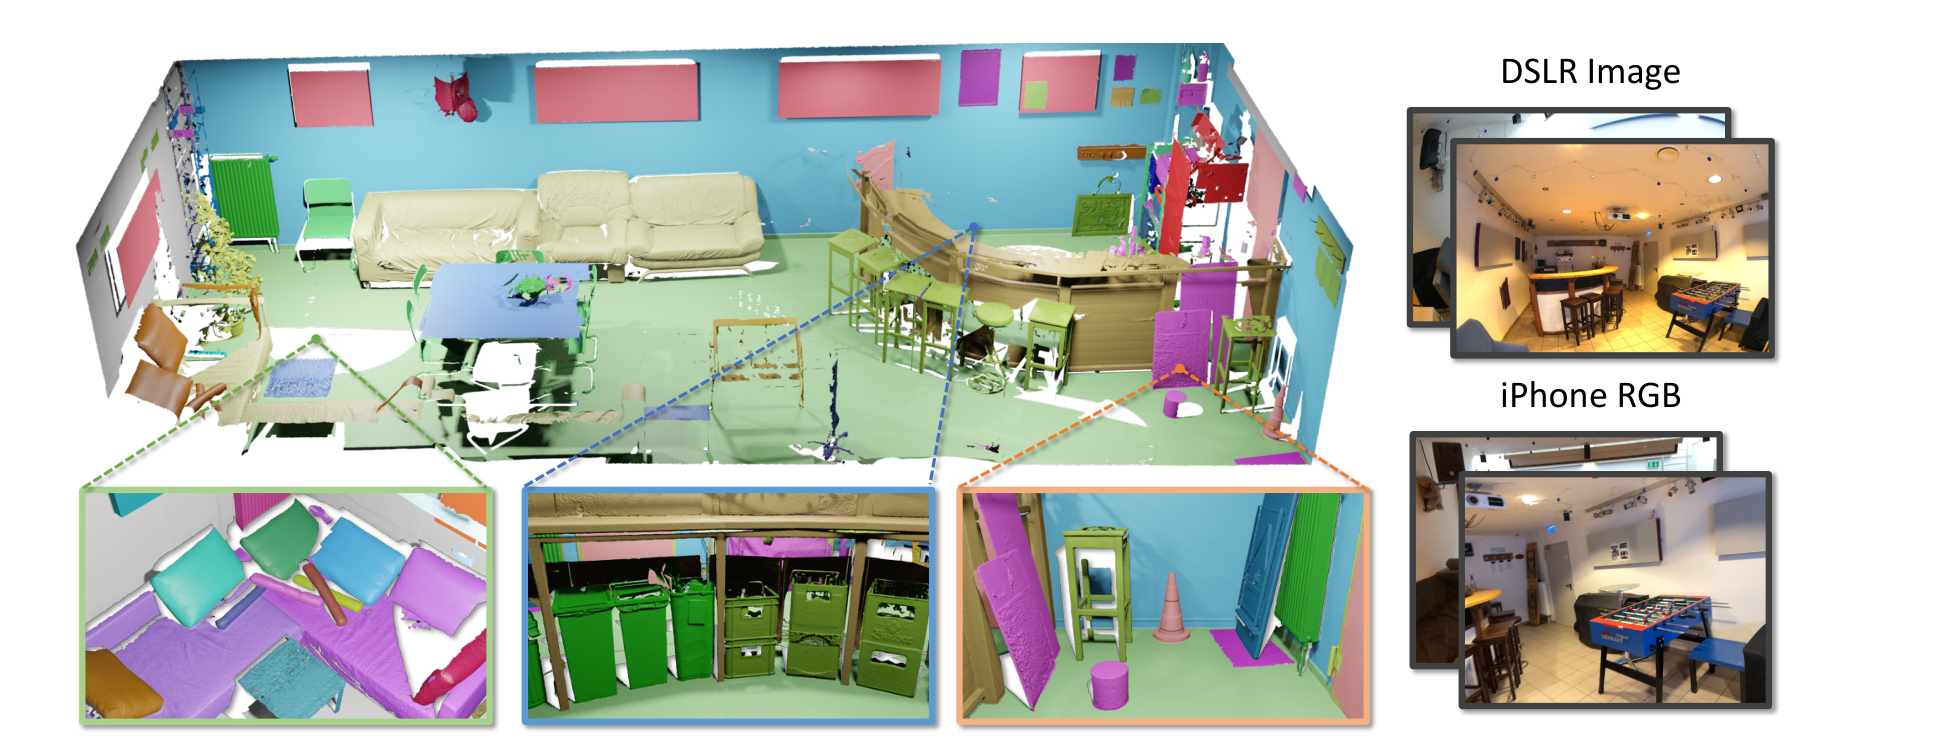
\includegraphics[width=0.95\linewidth]{scannetpp_overview_crop.png}
    \caption{Overview of the dataset environment showing the diversity of indoor scenes and the dense 3D ground truth structure, adapted from the ScanNet dataset paper/project page~\cite{scannet}.}
    \label{fig:scannet_overview}
\end{figure}

To simulate a realistic sparse-view deployment scenario, our input data is strictly limited to small groups of 3 to 5 RGB views sampled from these scenes. Figure \ref{fig:dataset_inputs} illustrates an example of the raw sparse RGB images provided to the system. Importantly, no external camera poses or active depth sensor measurements are provided to the pipeline during the inference phase.

\begin{figure}[H]
    \centering
    \begin{subfigure}[b]{0.31\textwidth}
        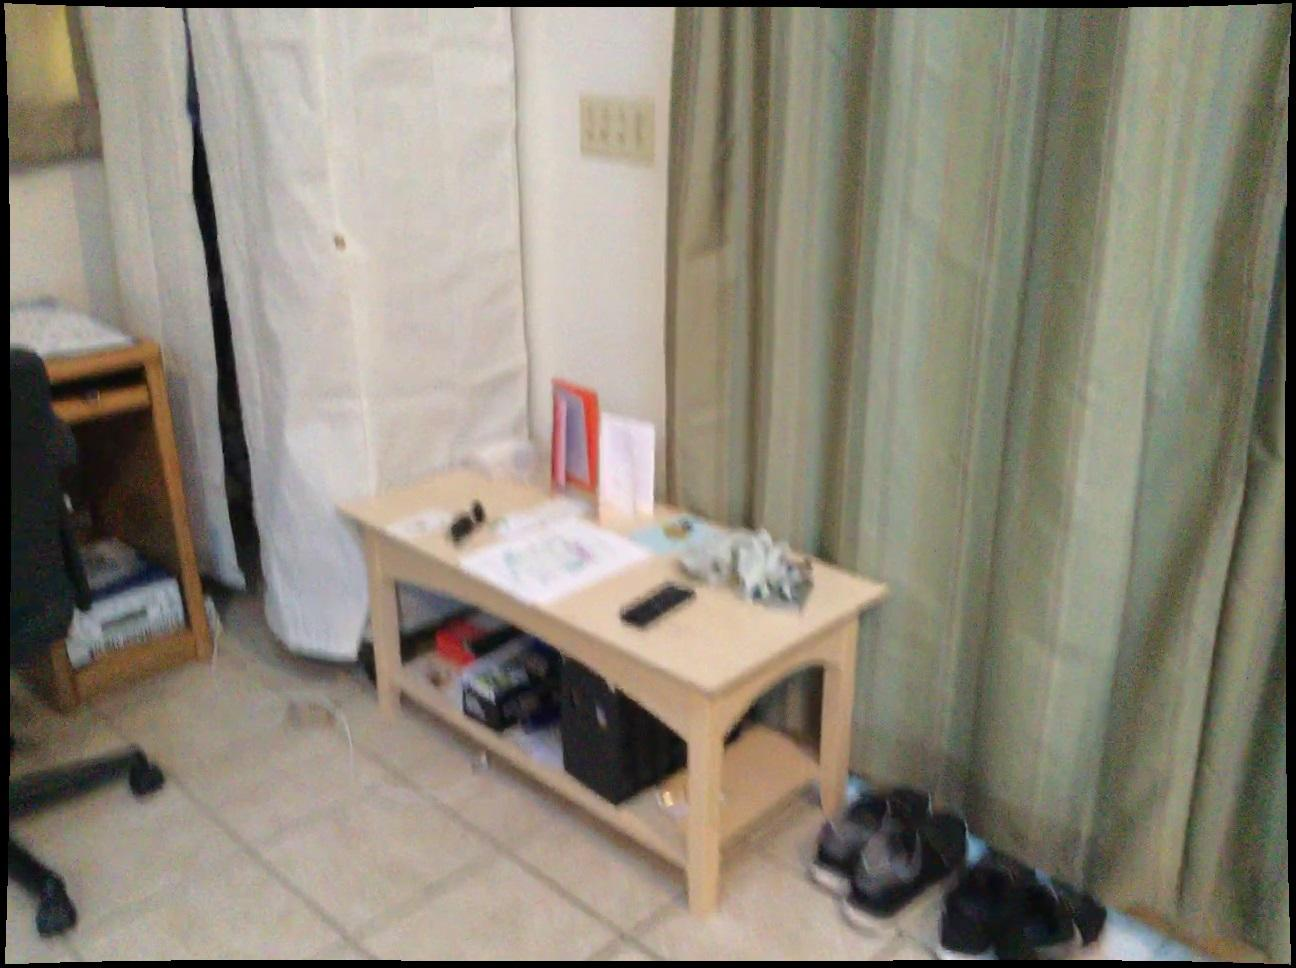
\includegraphics[width=\textwidth]{sparse_rgb_input_scene0000_00_view1.jpg}
        \caption{Input view 1}
    \end{subfigure}
    \hfill
    \begin{subfigure}[b]{0.31\textwidth}
        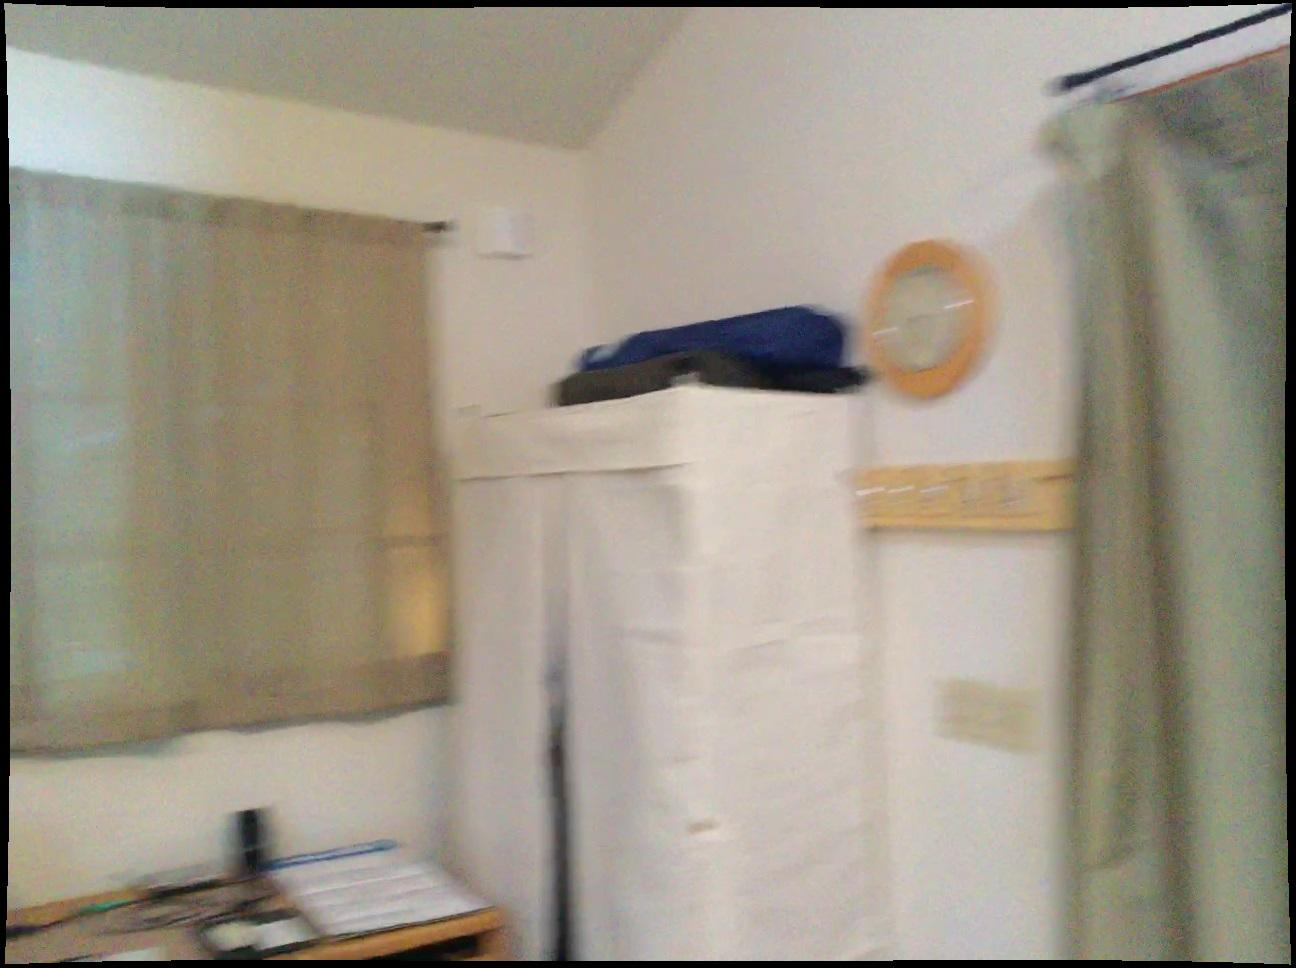
\includegraphics[width=\textwidth]{sparse_rgb_input_scene0000_00_view2.jpg}
        \caption{Input view 2}
    \end{subfigure}
    \hfill
    \begin{subfigure}[b]{0.31\textwidth}
        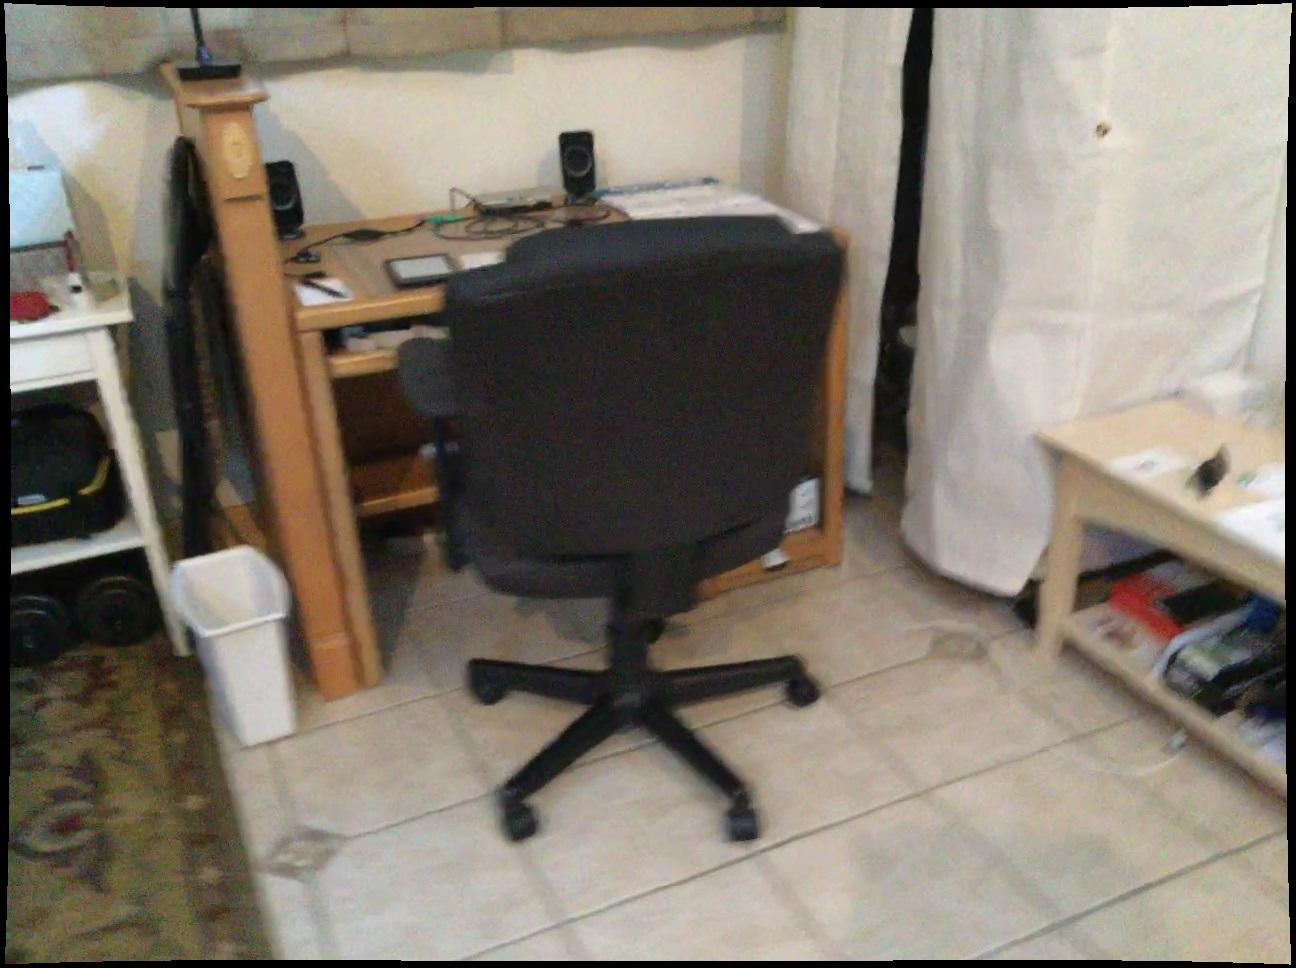
\includegraphics[width=\textwidth]{sparse_rgb_input_scene0000_00_view3.jpg}
        \caption{Input view 3}
    \end{subfigure}
    \vspace{0.35cm}
    \begin{subfigure}[b]{0.78\textwidth}
        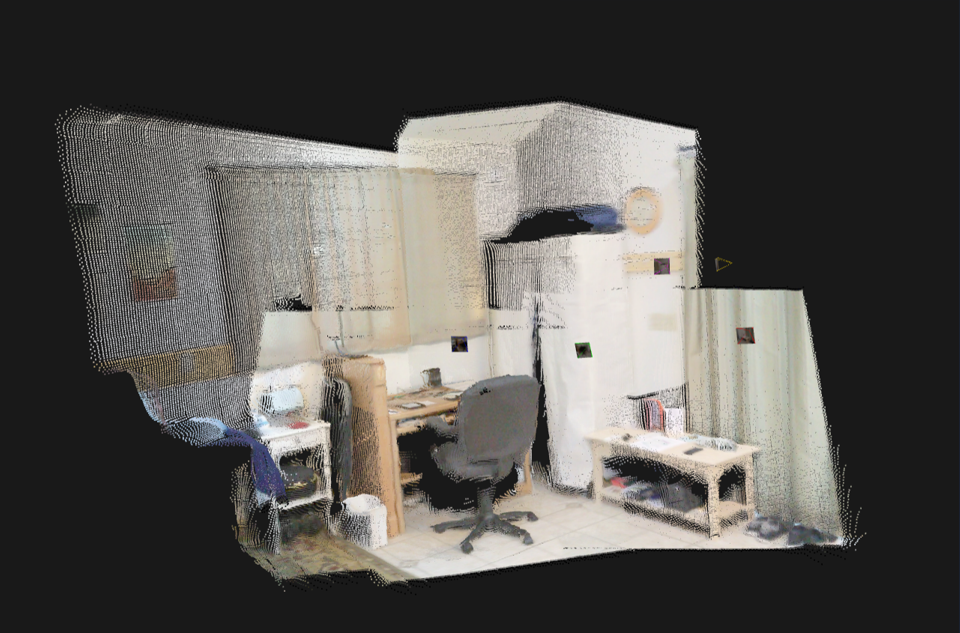
\includegraphics[width=\textwidth]{sparse_rgb_scene0000_00_pointcloud_preview.png}
        \caption{Example reconstructed point cloud preview}
    \end{subfigure}
    \caption{Example sparse RGB input views and the corresponding 3D point-cloud visualization from the project experiments. The system receives only sparse RGB images at inference time and must infer both scene geometry and depth cues from these limited viewpoints.}
    \label{fig:dataset_inputs}
\end{figure}

For quantitative evaluation and depth estimator fine-tuning, the dataset also includes aligned RGB-D ground truth information. Figure \ref{fig:3d_gt} displays an example of the measured 3D ground truth structure, which is used strictly as an upper-bound reference to compute Chamfer distance and F-score reconstruction metrics.

\begin{figure}[H]
    \centering
    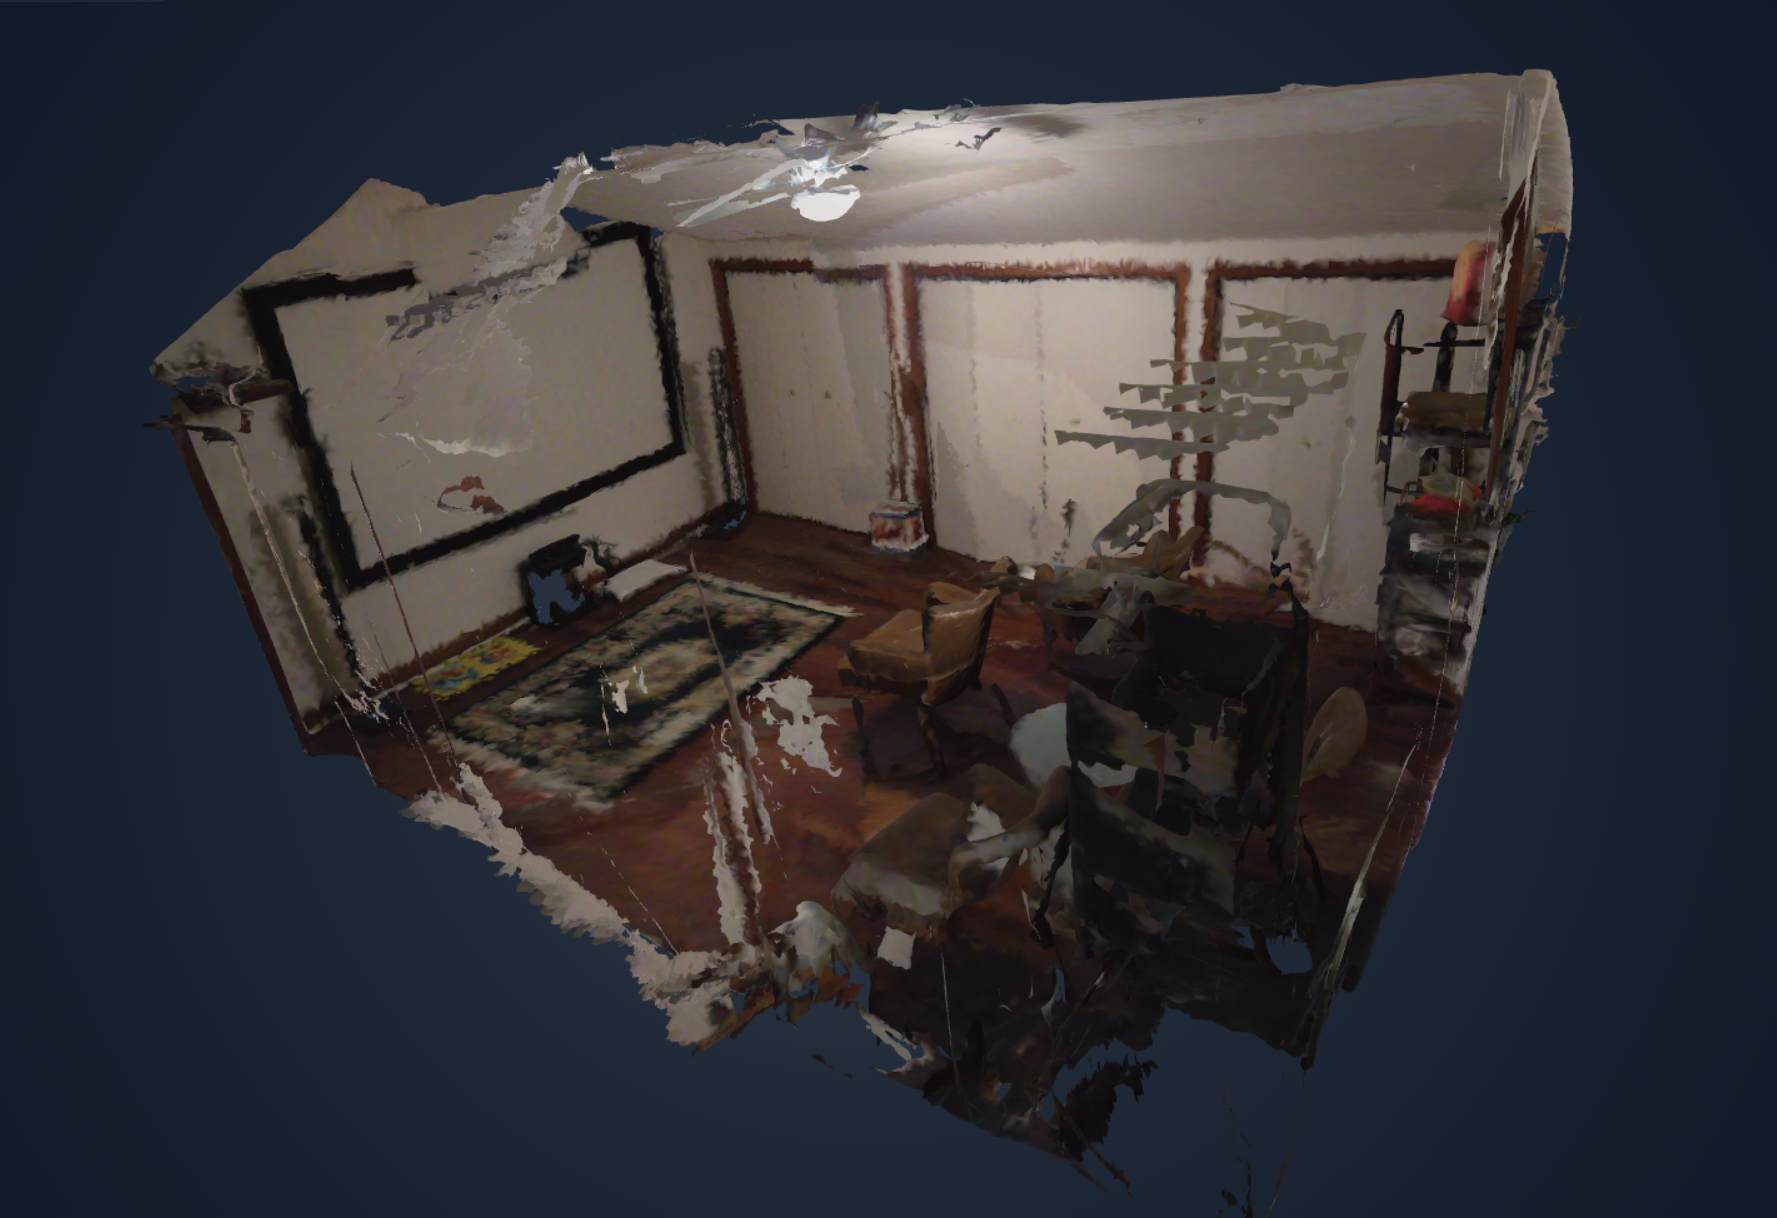
\includegraphics[width=0.6\linewidth]{3D_GT.png}
    \caption{Example of a 3D Ground Truth point cloud used for quantitative metric evaluation.}
    \label{fig:3d_gt}
\end{figure}

\subsection{Experimental Setting}
The experiments are designed to strictly evaluate the sparse-view RGB-only deployment scenario. The primary 3D reconstruction backbone is \mvdp{}, which receives groups of \(N = 3\) to \(5\) unposed RGB images to generate initial multi-view candidate geometry.

For depth estimation, the \da{} model is employed. To improve its reliability on complex indoor structures and resolve metric scale ambiguity, the model is fine-tuned on the measured RGB-D data from the training split. During inference, this fine-tuned depth estimator processes the sparse RGB views independently to generate metric depth priors.

The diagnostic correction module then attempts to combine the rigid camera poses extracted from the \mvdp{} output with the fine-tuned metric depth anchors. A geometric correction algorithm is applied to test whether structurally distorted candidate points can be pulled toward the physical surfaces suggested by the metric depth rays.

All inferences and fine-tuning processes are executed in a controlled Kaggle notebook environment equipped with NVIDIA GPUs. The system ultimately outputs reconstructed 3D point clouds in a common coordinate frame for downstream 3D visualization and quantitative evaluation.

\subsection{Compared Methods}
The evaluation compares four reconstruction settings that isolate the role of each component:
\begin{enumerate}[leftmargin=1.2cm]
    \item \textbf{RGB-only \mvdp{}.} This is the multi-view baseline. It uses only sparse RGB images and no estimated-depth correction.
    \item \textbf{Direct estimated-depth backprojection.} This removes \mvdp{} candidate point geometry and reconstructs 3D directly from the fine-tuned estimated depth and the camera geometry recovered by \mvdp{}.
    \item \textbf{Correction with pretrained estimated depth.} This tests whether an off-the-shelf monocular depth model is already reliable enough to correct \mvdp{} points.
    \item \textbf{Correction with fine-tuned estimated depth.} This is the intended main diagnostic setting. It uses \mvdp{} candidate geometry together with the fine-tuned depth estimator.
\end{enumerate}
All four settings are evaluated on the same sparse-view groups so that the comparison reflects the reconstruction method rather than a change in input images.

% ------------------------------------------------------------------
\section{Evaluation Metrics}
\subsection{Depth Estimation Metrics}
Let \(D\) be the measured depth map and \(\hat{D}\) be the predicted depth map over valid pixels \(\Omega\). The depth metrics are:
\begin{align}
\mathrm{AbsRel} &= \frac{1}{|\Omega|}\sum_{p\in\Omega}\frac{|D(p)-\hat{D}(p)|}{D(p)},\\
\mathrm{MAE} &= \frac{1}{|\Omega|}\sum_{p\in\Omega}|D(p)-\hat{D}(p)|,\\
\mathrm{RMSE} &= \sqrt{\frac{1}{|\Omega|}\sum_{p\in\Omega}\left(D(p)-\hat{D}(p)\right)^2}.
\end{align}
The \(\delta_1\) accuracy is the fraction of pixels satisfying:
\begin{equation}
\max\left(\frac{\hat{D}(p)}{D(p)},\frac{D(p)}{\hat{D}(p)}\right)<1.25.
\end{equation}
Lower AbsRel, MAE, and RMSE are better, while higher \(\delta_1\) is better.

\subsection{Point-Cloud Reconstruction Metrics}
Let \(P\) be the predicted point cloud and \(G\) be the reference point cloud. Accuracy is the average nearest-neighbor distance from prediction to reference:
\begin{equation}
\mathrm{Accuracy}=\frac{1}{|P|}\sum_{p\in P}\min_{g\in G}\|p-g\|_2.
\end{equation}
Completeness is the average nearest-neighbor distance from reference to prediction:
\begin{equation}
\mathrm{Completeness}=\frac{1}{|G|}\sum_{g\in G}\min_{p\in P}\|g-p\|_2.
\end{equation}
Precision and recall are computed at a fixed metric distance threshold. In the main reconstruction evaluation, this threshold is set to \(\tau_m=0.05\,\mathrm{m}\). F-score is:
\begin{equation}
F_1=\frac{2\cdot \mathrm{Precision}\cdot \mathrm{Recall}}{\mathrm{Precision}+\mathrm{Recall}}.
\end{equation}
Chamfer distance is:
\begin{equation}
\mathrm{Chamfer}=\mathrm{Accuracy}+\mathrm{Completeness}.
\end{equation}

For shape-level analysis, the project also reports Normalized Distance (ND) and the DAc@0.2 metric on selected qualitative groups. These metrics are computed after scale and center normalization and should not be interpreted as absolute metric-pose evaluation.

% ------------------------------------------------------------------
\section{Results}
\subsection{Depth Estimator Fine-Tuning}
Depth evaluation checks whether the fine-tuned depth estimator is accurate enough to serve as a correction anchor. The values in Table~\ref{tab:depthtrain} and Table~\ref{tab:depthmetrics} are taken from the depth-estimator fine-tuning experiment. The checkpoint used for held-out reporting is \texttt{controlled\_best}. The \texttt{full\_dataset\_deployment} checkpoint is a deployment artifact because it is trained again on all discovered frames.

\begin{table}[H]
\centering
\small
\renewcommand{\arraystretch}{1.18}
\resizebox{\linewidth}{!}{%
\begin{tabular}{@{}lrrrrrr@{}}
\toprule
Stage & Scenes & Training frames & Epochs & Mini-batch steps & Mean train loss & Elapsed time \\
\midrule
Controlled train split & 1210 & 198862 & 1 & 99431 & 0.0850 & 4.01 h \\
Full-data deployment & 1513 & 248402 & 1 & 124201 & 0.0718 & 4.08 h \\
\bottomrule
\end{tabular}%
}
\caption{Depth-estimator fine-tuning workload. The controlled stage uses the training split to select \texttt{controlled\_best}; the full-data stage uses all discovered scenes to create the deployment checkpoint.}
\label{tab:depthtrain}
\end{table}

\begin{table}[H]
\centering
\small
\renewcommand{\arraystretch}{1.18}
\resizebox{\linewidth}{!}{%
\begin{tabular}{@{}lcccccc@{}}
\toprule
Depth model & AbsRel $\downarrow$ & MAE (m) $\downarrow$ & RMSE (m) $\downarrow$ & $\delta_1$ $\uparrow$ & Scale-aligned MAE $\downarrow$ & Split \\
\midrule
Pretrained \da{} Metric Indoor & 0.2730 & 0.3839 & 0.4778 & 0.6441 & 0.1672 & validation \\
Fine-tuned \texttt{controlled\_best} & \textbf{0.1145} & \textbf{0.1431} & \textbf{0.2393} & \textbf{0.9355} & \textbf{0.0992} & validation \\
Pretrained \da{} Metric Indoor & 0.2707 & 0.3850 & 0.4806 & 0.6486 & 0.1676 & test \\
Fine-tuned \texttt{controlled\_best} & \textbf{0.1140} & \textbf{0.1428} & \textbf{0.2370} & \textbf{0.9362} & \textbf{0.0982} & test \\
\bottomrule
\end{tabular}%
}
\caption{Held-out depth evaluation. Each split uses 1200 sampled frames; validation contains 149 scenes and test contains 152 scenes.}
\label{tab:depthmetrics}
\end{table}

Fine-tuning substantially improves depth quality. On validation, AbsRel decreases from 0.2730 to 0.1145, MAE decreases from 0.3839 m to 0.1431 m, and \(\delta_1\) increases from 0.6441 to 0.9355. On test, AbsRel decreases from 0.2707 to 0.1140, MAE decreases from 0.3850 m to 0.1428 m, and \(\delta_1\) increases from 0.6486 to 0.9362. This indicates that the fine-tuned depth estimator is much more reliable than the initial pretrained checkpoint on the controlled ScanNet-style indoor subset.

\begin{figure}[H]
    \centering
    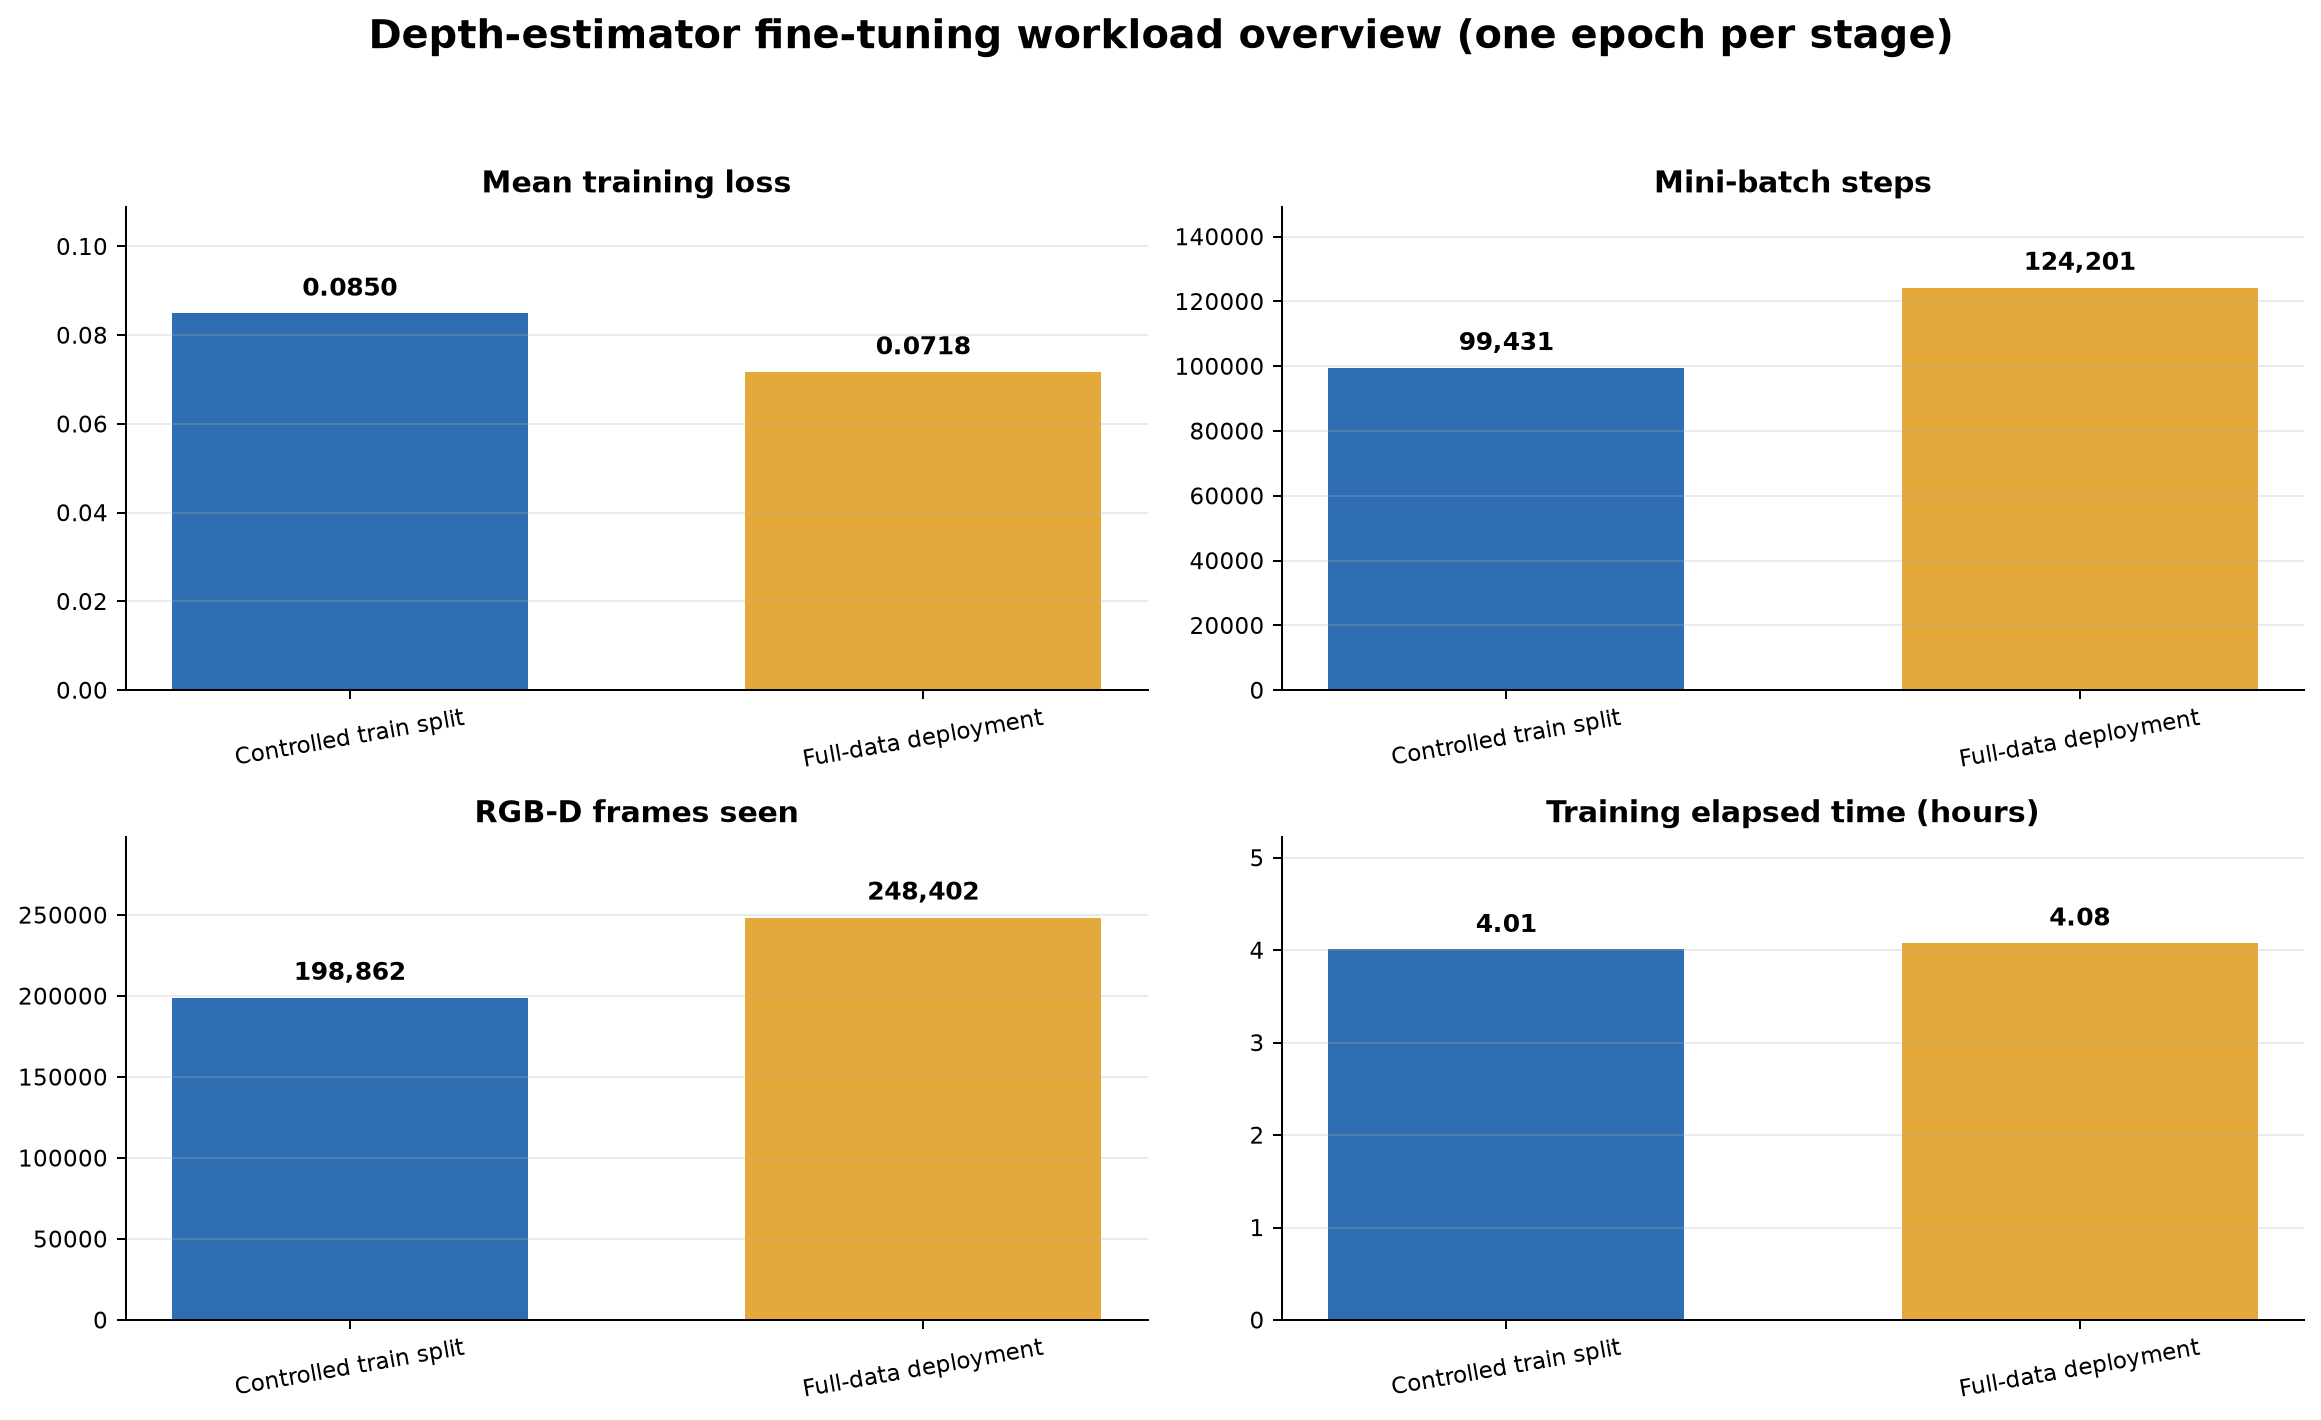
\includegraphics[width=0.92\linewidth]{depth_finetune_training_overview.png}
    \caption{Fine-tuning workload overview. Because the experiment logs one epoch per stage, this figure should be interpreted as a workload, mean-loss, and elapsed-time summary rather than as a multi-epoch training-loss curve.}
    \label{fig:depth_finetune_training_overview}
\end{figure}

\begin{figure}[H]
    \centering
    \begin{subfigure}{0.96\linewidth}
        \centering
        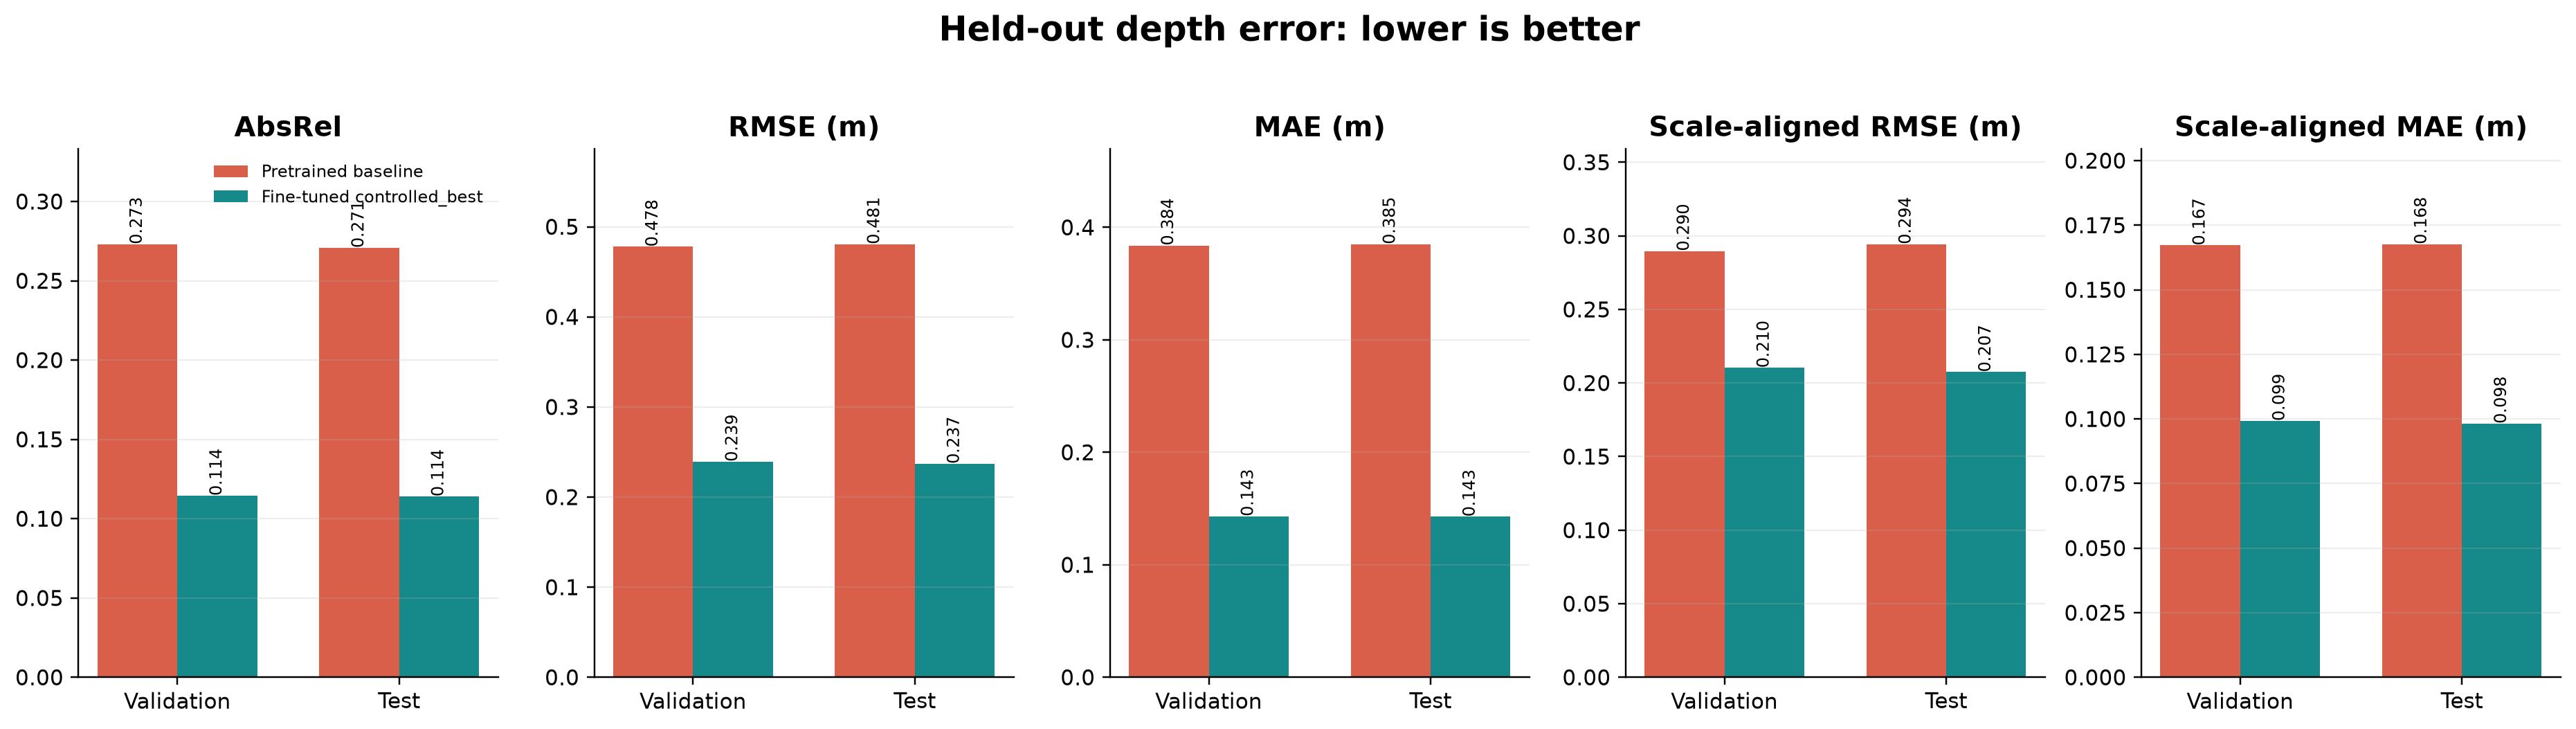
\includegraphics[width=\linewidth]{depth_finetune_eval_error_metrics.png}
        \caption{Depth error metrics on validation/test.}
    \end{subfigure}
    \vspace{0.35cm}
    \begin{subfigure}{0.78\linewidth}
        \centering
        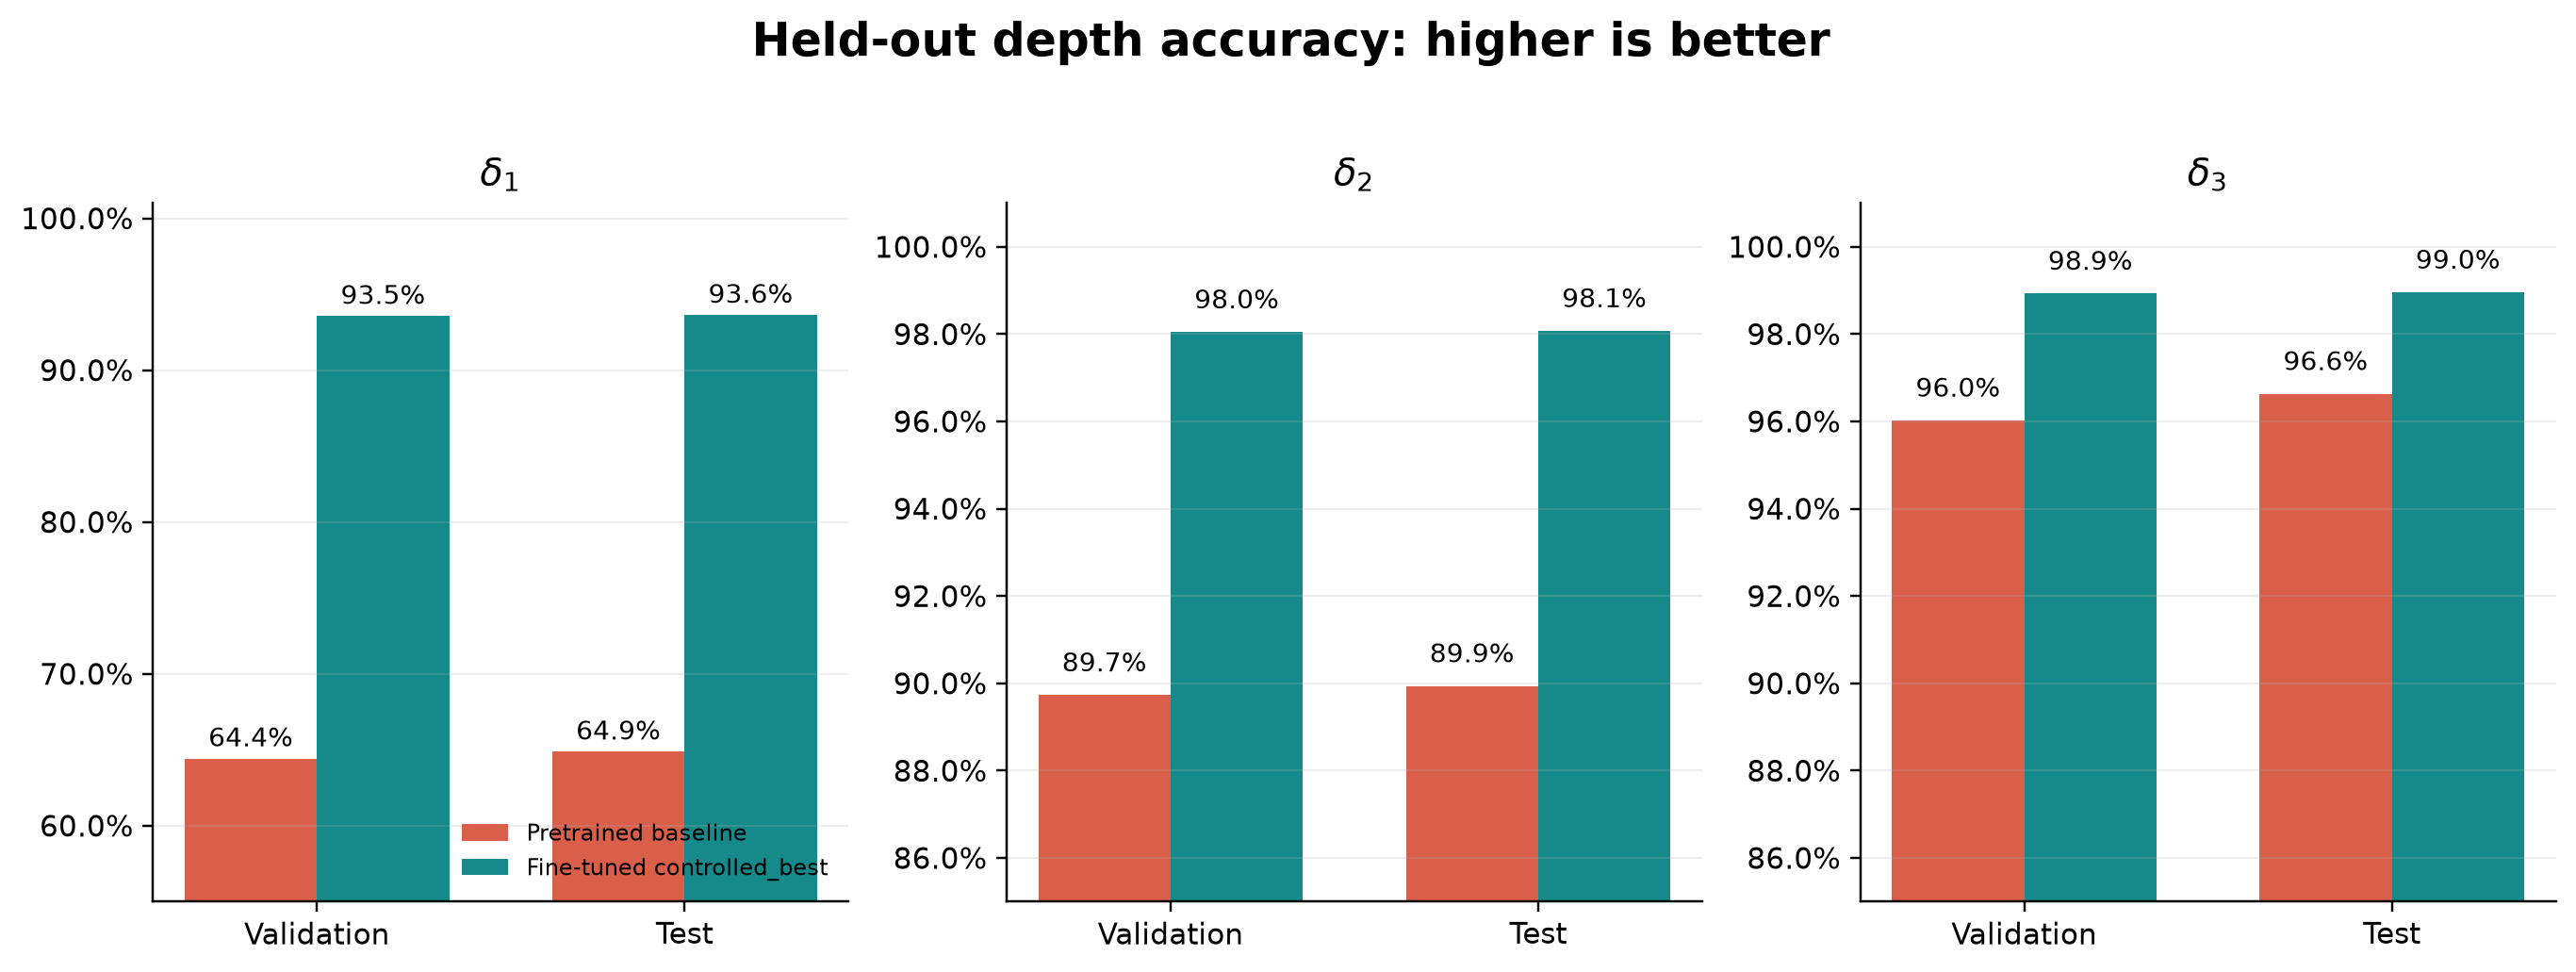
\includegraphics[width=\linewidth]{depth_finetune_eval_accuracy_metrics.png}
        \caption{Depth accuracy metrics \(\delta_1\), \(\delta_2\), and \(\delta_3\).}
    \end{subfigure}
    \caption{Comparison between the pretrained checkpoint and the fine-tuned \texttt{controlled\_best} checkpoint.}
    \label{fig:depth_finetune_eval_metrics}
\end{figure}

\begin{figure}[H]
    \centering
    \begin{subfigure}{0.92\linewidth}
        \centering
        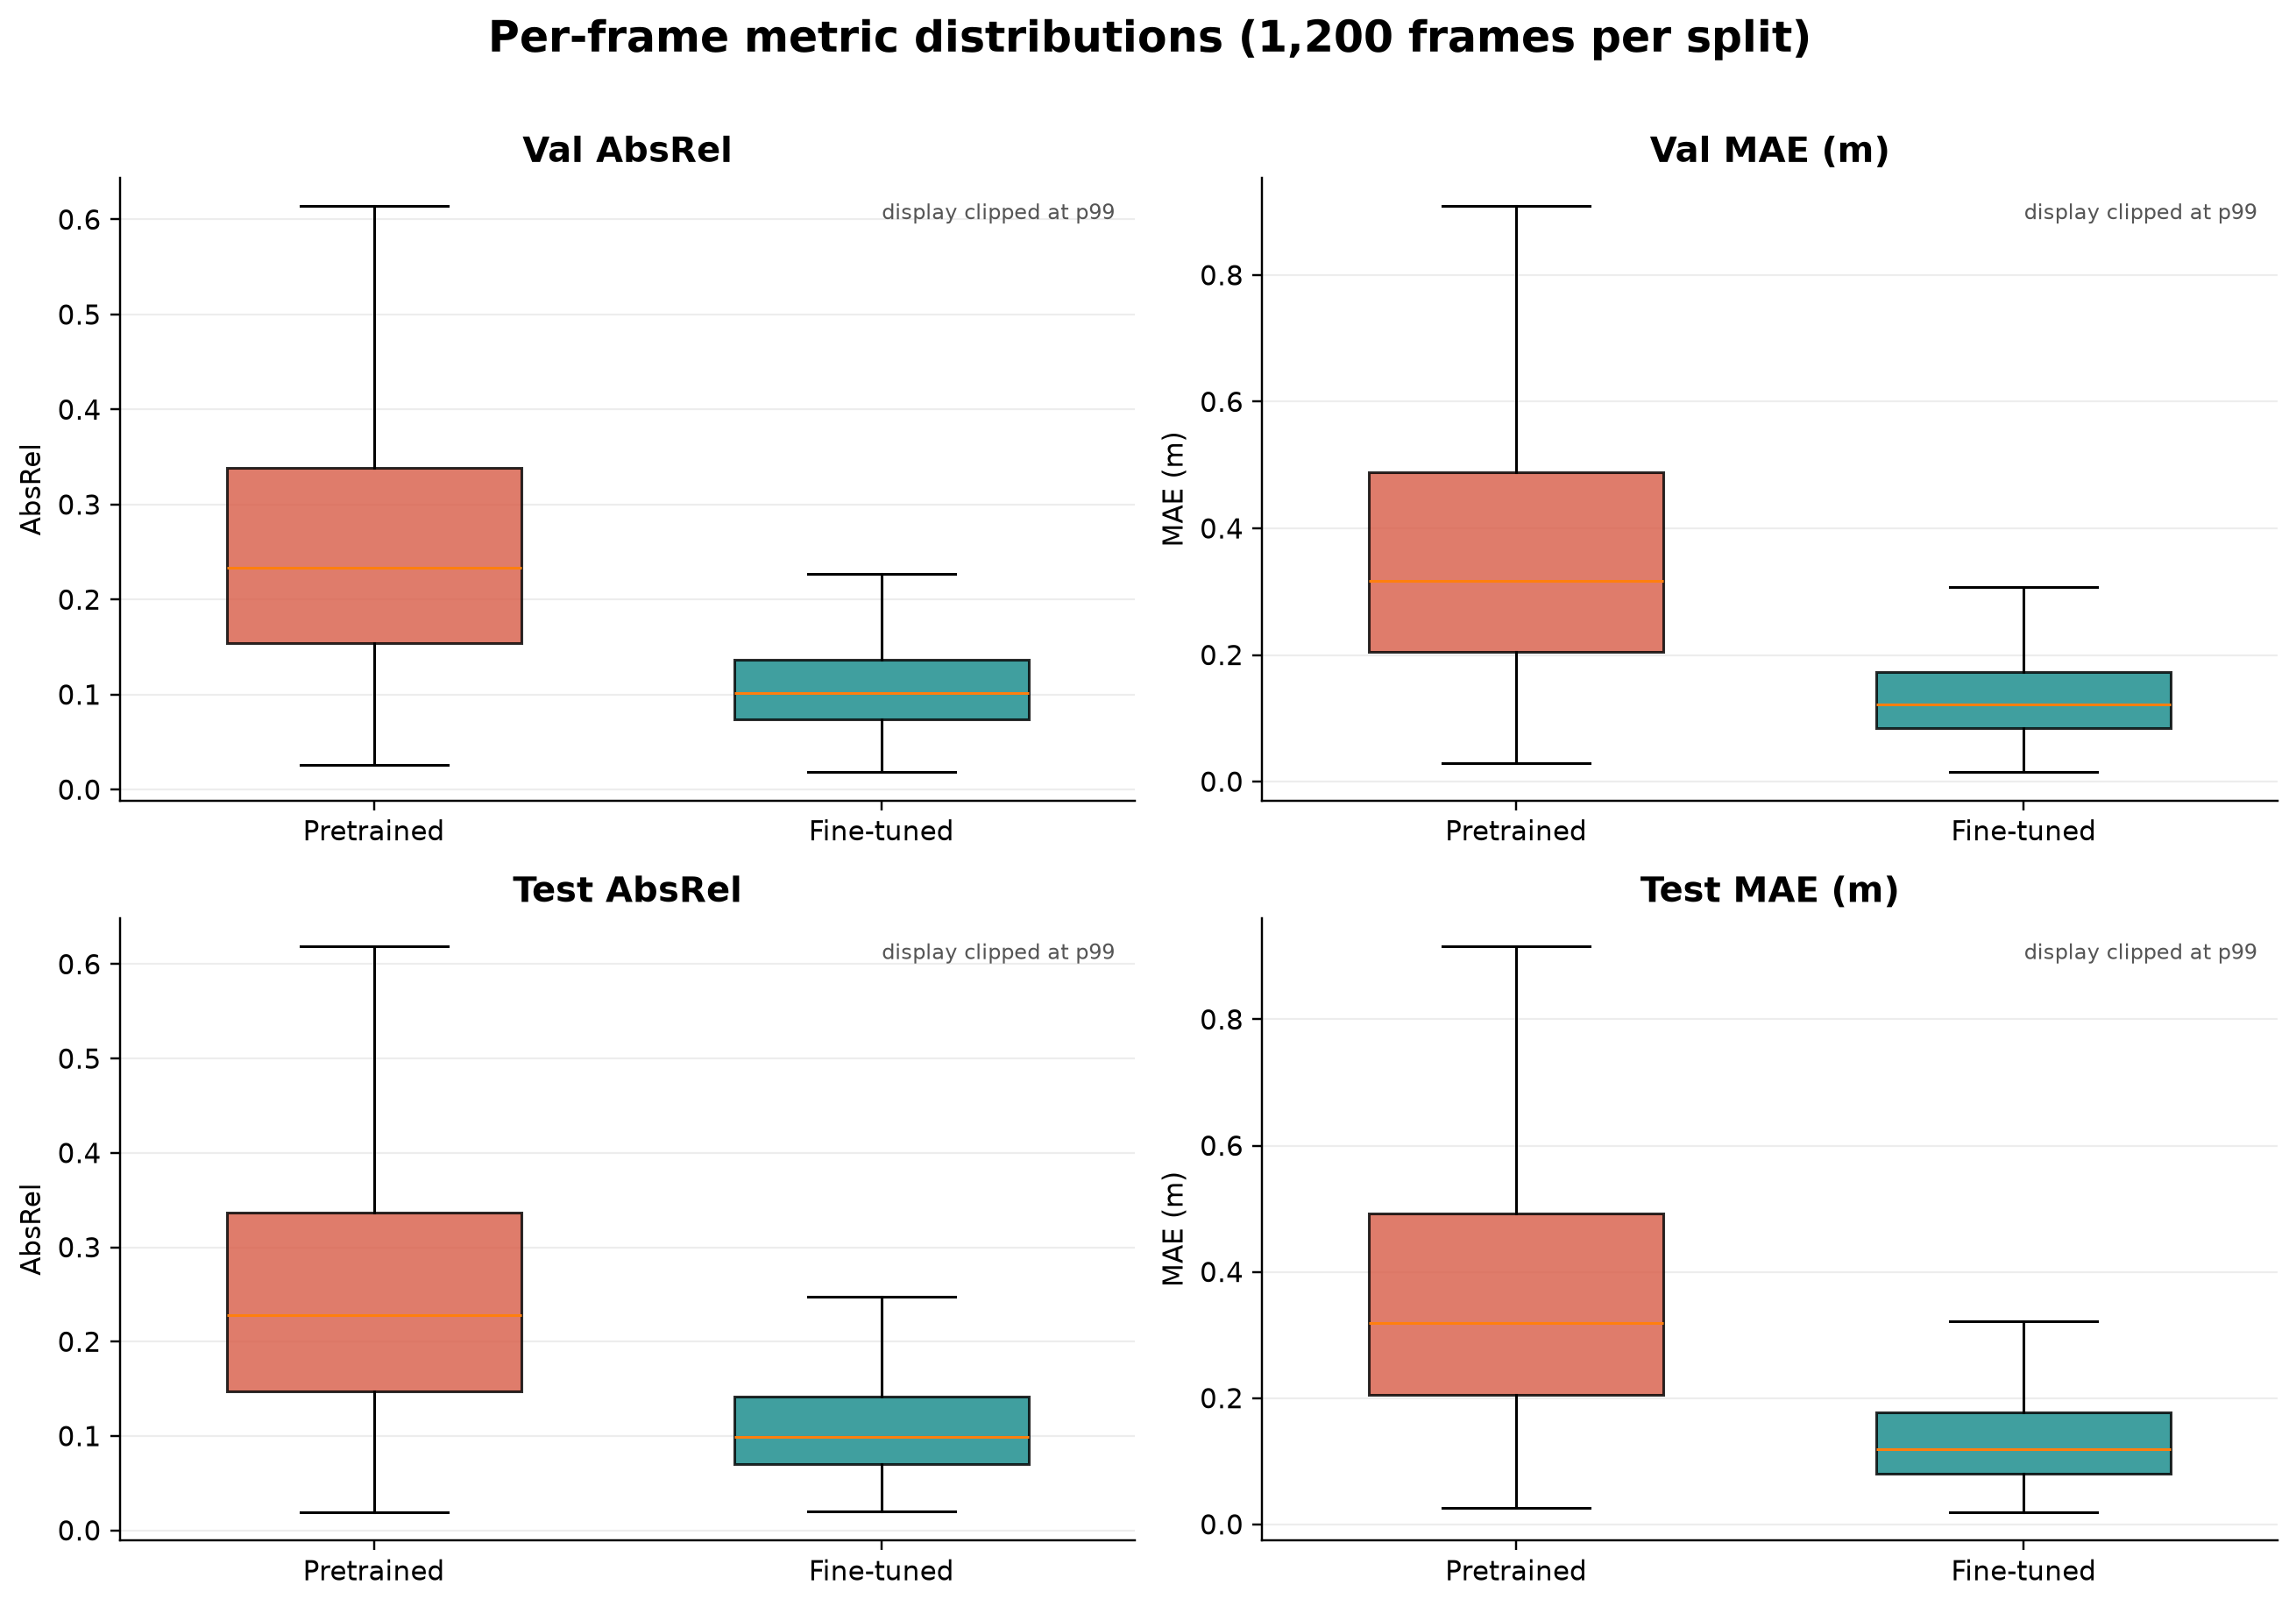
\includegraphics[width=\linewidth]{depth_finetune_per_frame_distributions.png}
        \caption{Per-frame distributions of depth metrics.}
    \end{subfigure}
    \vspace{0.35cm}
    \begin{subfigure}{0.82\linewidth}
        \centering
        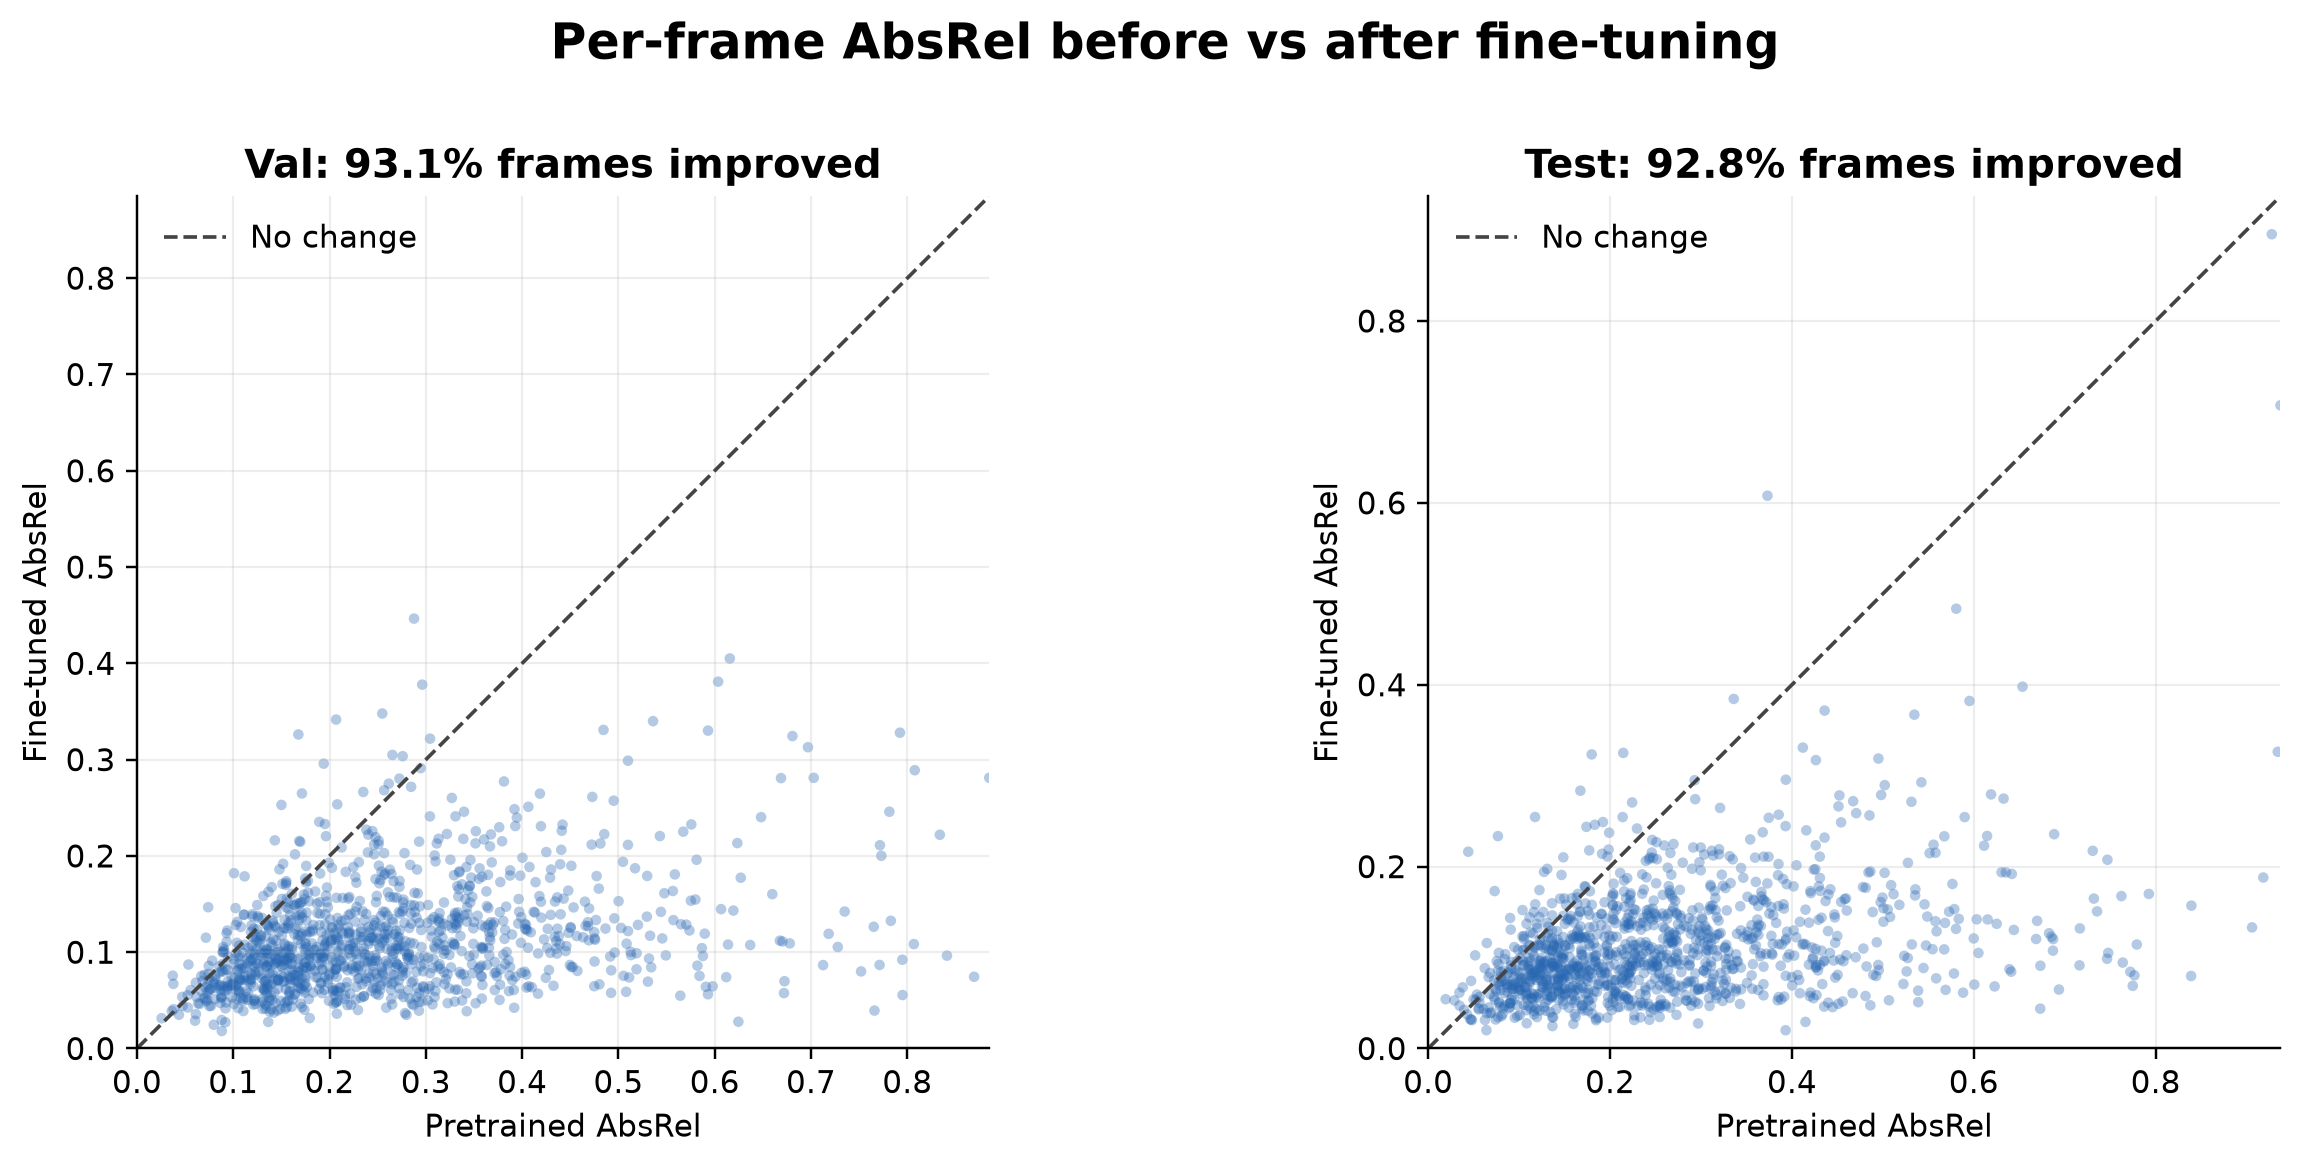
\includegraphics[width=\linewidth]{depth_finetune_absrel_scatter.png}
        \caption{AbsRel scatter before and after fine-tuning.}
    \end{subfigure}
    \caption{Per-frame analysis shows that the gain is not caused by a few easy frames. The fine-tuned checkpoint reduces AbsRel on about 93.1\% of validation frames and 92.8\% of test frames.}
    \label{fig:depth_finetune_per_frame}
\end{figure}

\subsection{3D Reconstruction Results}
The main reconstruction experiment evaluates the hypothesis that estimated-depth correction can improve over RGB-only \mvdp{}. Table~\ref{tab:recon} summarizes completed controlled experiments. These values use the project controlled sparse-view protocol and should not be interpreted as official full ScanNet or ScanNet++ benchmark results.

\begin{table}[H]
\centering
\small
\renewcommand{\arraystretch}{1.18}
\resizebox{\linewidth}{!}{%
\begin{tabular}{@{}lcccccc@{}}
\toprule
Method & Accuracy $\downarrow$ & Completeness $\downarrow$ & Precision $\uparrow$ & Recall $\uparrow$ & F-score $\uparrow$ & Chamfer $\downarrow$ \\
\midrule
\textbf{RGB-only \mvdp{} (best observed)} & \textbf{0.1627} & \textbf{0.1641} & \textbf{0.4029} & \textbf{0.6834} & \textbf{0.5069} & \textbf{0.3268} \\
Direct backprojection from estimated depth & 0.2037 & 0.2041 & 0.2029 & 0.1834 & 0.1927 & 0.4078 \\
Correction with pretrained estimated depth & 0.2440 & 0.2655 & 0.1307 & 0.1043 & 0.1160 & 0.5095 \\
\textit{Correction with fine-tuned estimated depth (intended main setting)} & 0.2240 & 0.2355 & 0.1707 & 0.1343 & 0.1503 & 0.4595 \\
\end{tabular}%
}
\caption{3D reconstruction comparison on completed test-group experiments. F-score is computed from the Precision and Recall values in the table. Bold values indicate the best observed result in this table. These values are controlled project metrics and should not be interpreted as official full ScanNet or ScanNet++ benchmark results.}
\label{tab:recon}
\end{table}

The initial expectation was that the intended main diagnostic setting, namely \textit{correction with fine-tuned estimated depth}, would be the strongest reconstruction setting. The motivation was straightforward: \mvdp{} should provide multi-view candidate geometry, while the fine-tuned depth estimator should provide metric depth anchors to correct wrong-depth regions. However, the completed experiment does not support this expectation. In Table~\ref{tab:recon}, the RGB-only \mvdp{} baseline remains the best observed method, with the highest F-score and the lowest reported Chamfer value.

By F-score, the observed order is: RGB-only \mvdp{} first, direct estimated-depth backprojection second, fine-tuned estimated-depth correction third, and pretrained estimated-depth correction last. This means that fine-tuning the depth estimator helps compared with the pretrained-depth correction variant, but the correction module still does not outperform the original \mvdp{} candidate reconstruction.

The most likely reason is that the correction stage is very sensitive to coordinate-frame and scale consistency. The correction formula assumes that the \mvdp{} candidate point, the estimated-depth anchor, the camera intrinsics, and the camera pose all describe the same metric 3D coordinate system. In practice, \mvdp{} produces geometry in its own reconstructed coordinate frame, while monocular estimated depth can still contain per-frame scale bias and local depth errors even after fine-tuning. The fine-tuned depth model improves the per-pixel MAE substantially, but its held-out MAE is still about 0.14 m, which is large relative to strict 3D reconstruction thresholds. Therefore, when the correction module pulls candidate points toward imperfect estimated-depth anchors, it can move already reasonable \mvdp{} points away from the reference surface and reduce precision.

This result should be interpreted as a negative but useful ablation. It does not mean that the fine-tuned depth estimator is useless: the depth metrics show a clear improvement after fine-tuning. Instead, it shows that the current residual-gated correction rule is not robust enough to combine \mvdp{} geometry and estimated depth reliably. A stronger final version would need confidence-aware correction, scale alignment between \mvdp{} and depth, and preferably ray-only correction that changes depth along each camera ray instead of freely moving world-space points.

\subsection{Ablation Study}
The ablation study answers three questions. First, comparing RGB-only \mvdp{} with pretrained-depth correction tests whether off-the-shelf monocular depth helps without task adaptation. Second, comparing pretrained-depth correction with fine-tuned-depth correction tests whether fine-tuning on RGB-D training data improves reconstruction. Third, comparing fine-tuned-depth correction with direct estimated-depth backprojection tests whether the current correction rule is actually better than using estimated depth alone.

The ablation result is informative. Pretrained-depth correction is the weakest setting, which confirms that using an unadapted monocular depth model as a hard correction anchor is harmful. Fine-tuned-depth correction improves over pretrained-depth correction, so fine-tuning does move the depth prior in the right direction. Nevertheless, direct estimated-depth backprojection is still stronger than the current correction variant, and RGB-only \mvdp{} is strongest overall in the completed table. This suggests that the bottleneck is not only depth quality, but also the geometric coupling between estimated depth, camera rays, and the \mvdp{} output coordinate frame.

\subsection{Qualitative Analysis}
The qualitative comparison presents reconstructed point clouds side by side for the same sparse-view scene group. It includes the RGB-only \mvdp{} point cloud, direct estimated-depth backprojection, correction with pretrained estimated depth, and correction with fine-tuned estimated depth.

The RGB-only baseline is visually the most coherent in this example. The direct and corrected variants preserve some room-level structure, but they also show stretched surfaces, noisy sheets near object boundaries, and stronger view-dependent distortion. These visual patterns are consistent with the quantitative table: improving the monocular depth estimator does not automatically guarantee a better fused 3D point cloud.

Figure~\ref{fig:qual_recon_comparison} provides a visual comparison on the same sparse-view scene used in the qualitative output folder. The RGB-only \mvdp{} result gives the multi-view candidate reconstruction, direct estimated-depth backprojection reconstructs the scene using the fine-tuned depth estimator without the \mvdp{} candidate geometry, and the two correction variants show how the candidate point cloud changes when the correction anchor comes from either the pretrained or fine-tuned depth estimator.

\begin{figure}[H]
    \centering
    \begin{subfigure}[b]{0.48\textwidth}
        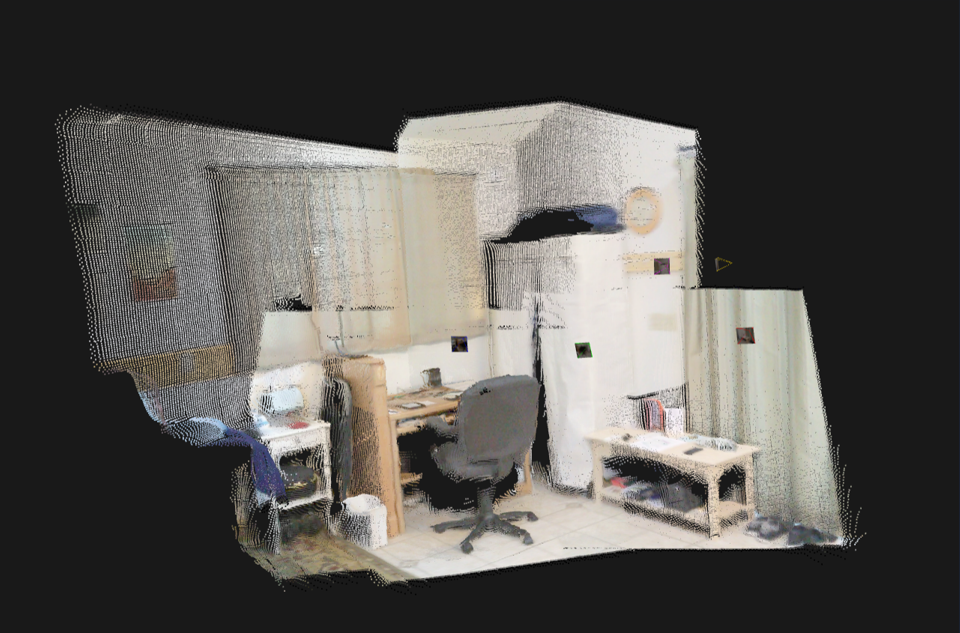
\includegraphics[width=\textwidth]{qual_rgb_only_mvdust3r.png}
        \caption{RGB-only \mvdp{}}
    \end{subfigure}
    \hfill
    \begin{subfigure}[b]{0.48\textwidth}
        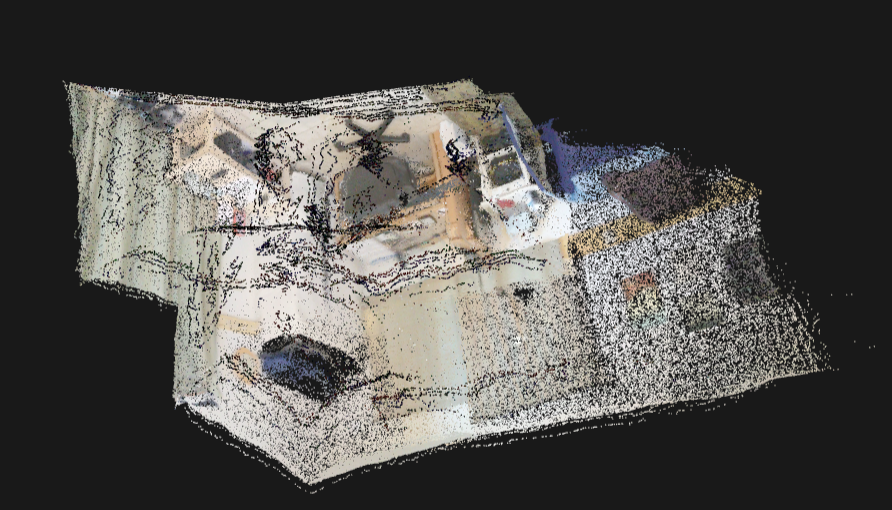
\includegraphics[width=\textwidth]{qual_direct_finetuned_depth.png}
        \caption{Direct backprojection from fine-tuned estimated depth}
    \end{subfigure}
    \vspace{0.35cm}
    \begin{subfigure}[b]{0.48\textwidth}
        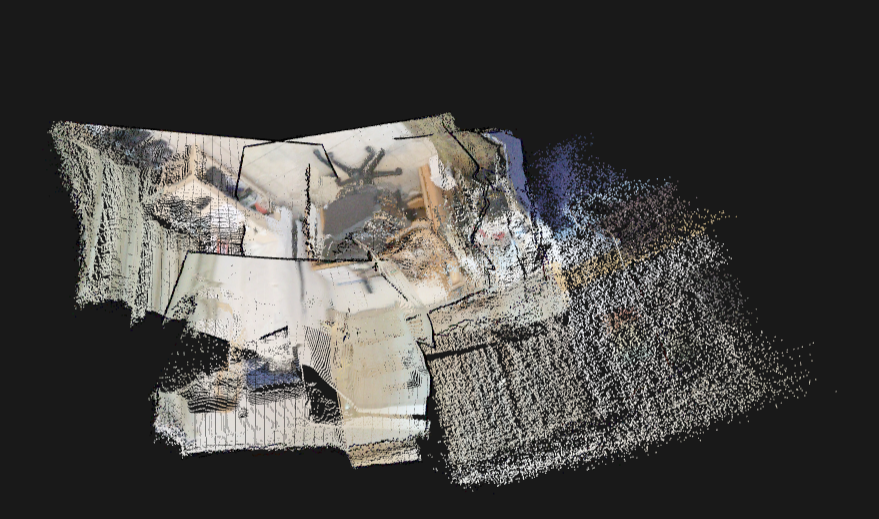
\includegraphics[width=\textwidth]{qual_correction_pretrained_depth.png}
        \caption{Correction with pretrained estimated depth}
    \end{subfigure}
    \hfill
    \begin{subfigure}[b]{0.48\textwidth}
        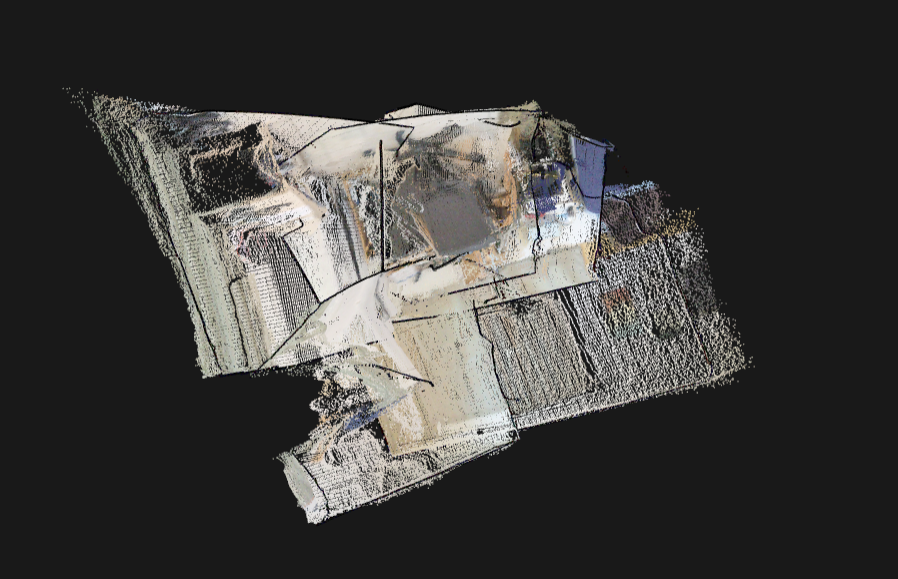
\includegraphics[width=\textwidth]{qual_correction_finetuned_depth.png}
        \caption{Correction with fine-tuned estimated depth}
    \end{subfigure}
    \caption{Qualitative comparison of the four reconstruction settings on the same sparse-view indoor scene.}
    \label{fig:qual_recon_comparison}
\end{figure}

\subsection{Failure Analysis}
The quantitative and qualitative results show that better monocular depth does not automatically produce a better 3D point cloud. The main failure mechanisms are:
\begin{enumerate}[leftmargin=1.2cm]
    \item \textbf{2.5D depth stretching.} A monocular depth map describes surfaces from one camera viewpoint. When it is directly back-projected into 3D, object boundaries and occlusion edges can become stretched surfaces or noisy depth sheets. This reduces precision because many projected points are geometrically plausible from the input view but inconsistent with the full 3D scene.
    \item \textbf{Camera-geometry errors are amplified.} Back-projection is highly sensitive to the camera pose and intrinsics. A small angular error in \(\hat{T}_i\) or a small focal-length error in \(\hat{K}_i\) can move distant points by a large amount in world coordinates. Therefore, even a good depth map can create misaligned 3D anchors if the camera geometry is not perfectly consistent with the \mvdp{} point cloud.
    \item \textbf{Forced blending can damage good multi-view geometry.} The \mvdp{} baseline often produces coherent structures through multi-view matching. If the estimated-depth anchor is slightly mis-scaled or misaligned, residual-gated blending can pull already reasonable candidate points away from the correct surface. In that case, the correction module breaks good geometry instead of fixing bad geometry.
\end{enumerate}

These failure modes explain why the fine-tuned depth model improves depth metrics but does not yet improve the final 3D reconstruction metrics. The next correction design should therefore be more selective: it should use depth confidence, \mvdp{} confidence, scale alignment, and preferably ray-only correction so that candidate points are adjusted along camera rays rather than moved freely in world space.

% ------------------------------------------------------------------
\section{Discussion}
This project is motivated by deployability. A system that requires measured depth at inference time can be accurate, but it is limited to users with specialized sensors. A system that only requires RGB images is easier to deploy because most cameras produce RGB images by default. Therefore, this project uses RGB-D data for training and evaluation while keeping the final inference input RGB-only.

This design also changes the interpretation of the dataset. The depth maps are not ignored. They are used as supervision for the depth estimator and as reference information for reconstruction evaluation. The final system then applies the learned depth knowledge to RGB-only inputs.

The original hypothesis was that estimated depth would improve geometric stability over RGB-only \mvdp{}. \mvdp{} provides multi-view candidate geometry but may still predict wrong depth in sparse-view settings, while the fine-tuned depth estimator provides a per-image geometric prior. The completed experiments show that this prior is useful at the depth-estimation level, but the current residual-gated fusion rule is not reliable enough to convert that prior into better final 3D reconstruction metrics. This motivates future work on confidence-aware and scale-aware depth correction.

The main limitation is that monocular depth is still imperfect. Fine-tuning reduces domain mismatch, but it does not remove all ambiguity. The depth model may still fail on unusual layouts, transparent objects, reflective surfaces, and scenes whose scale distribution differs from the training data. Therefore, final claims should remain limited to the controlled sparse-view RGB-only setting and should not be presented as an official ScanNet or ScanNet++ benchmark unless the official protocol is implemented.

% ------------------------------------------------------------------
\section{Conclusion}
This project studies sparse-view RGB-only 3D scene reconstruction from a small number of ordinary 2D images. The motivation is practical: most everyday images do not include measured depth, and requiring a depth sensor would reduce deployability. The project therefore uses measured RGB-D data for supervision and evaluation, but not as an inference-time input.

The diagnostic pipeline combines \mvdp{} with a fine-tuned monocular depth estimator. \mvdp{} produces candidate multi-view geometry from sparse RGB views, while the depth estimator predicts pseudo-depth maps from the same RGB inputs. The estimated-depth correction module is designed to refine candidate geometry, but the completed experiments show that the current residual-gated correction rule is not yet robust enough to outperform the RGB-only \mvdp{} baseline.

The report defines an evaluation framework for this setting. Depth quality is measured using monocular depth metrics. 3D reconstruction quality is measured using accuracy, completeness, precision, recall, F-score, and Chamfer distance. The compared settings are the RGB-only \mvdp{} baseline, direct estimated-depth backprojection, correction with pretrained estimated depth, and correction with fine-tuned estimated depth. The fine-tuned correction result should therefore be interpreted as a diagnostic finding: depth fine-tuning helps the depth prior, but fusion reliability remains the key limitation.

Future work should improve scale alignment between \mvdp{} geometry and estimated depth, add confidence-aware ray-based correction, evaluate more sparse-view groups, and test the method on more diverse real RGB image sets. The long-term goal is a deployable reconstruction system that can produce useful 3D scene geometry from only a few ordinary 2D images.

% ------------------------------------------------------------------
\newpage
\begin{thebibliography}{99}
\bibitem{mvdust3r_paper} Z. Tang, Y. Fan, D. Wang, H. Xu, R. Ranjan, A. Schwing, and Z. Yan, ``MV-DUSt3R+: Single-Stage Scene Reconstruction from Sparse Views in 2 Seconds,'' \textit{CVPR}, 2025. Available: \url{https://openaccess.thecvf.com/content/CVPR2025/papers/Tang_MV-DUSt3R_Single-Stage_Scene_Reconstruction_from_Sparse_Views_In_2_Seconds_CVPR_2025_paper.pdf}
\bibitem{mvdust3r_project} Meta Reality Labs, ``MV-DUSt3R+ official implementation,'' GitHub. Available: \url{https://github.com/facebookresearch/mvdust3r}
\bibitem{dust3r_paper} S. Wang, V. Leroy, Y. Cabon, B. Chidlovskii, and J. Revaud, ``DUSt3R: Geometric 3D Vision Made Easy,'' \textit{CVPR}, 2024. Available: \url{https://arxiv.org/abs/2312.14132}
\bibitem{mast3r_paper} V. Leroy, Y. Cabon, and J. Revaud, ``Grounding Image Matching in 3D with MASt3R,'' 2024. Available: \url{https://arxiv.org/abs/2406.09756}
\bibitem{depthanything_project} L. Yang et al., ``Depth Anything V2,'' \textit{NeurIPS}, 2024. Project page: \url{https://depth-anything-v2.github.io/}
\bibitem{depthanything_metric} Depth Anything V2, ``Metric depth estimation README,'' GitHub. Available: \url{https://github.com/depthanything/depth-anything-v2/blob/main/metric_depth/README.md}
\bibitem{scannet} A. Dai, A. X. Chang, M. Savva, M. Halber, T. Funkhouser, and M. Niessner, ``ScanNet: Richly-annotated 3D Reconstructions of Indoor Scenes,'' \textit{CVPR}, 2017. Dataset page: \url{https://www.scan-net.org/ScanNet/}
\bibitem{rsa_depth} Z. Zeng et al., ``RSA: Resolving Scale Ambiguities in Monocular Depth Estimators through Language Descriptions,'' arXiv:2410.02924, 2024. Available: \url{https://arxiv.org/abs/2410.02924}
\bibitem{mde_survey} C. Zhao, Q. Sun, C. Zhang, Y. Tang, and F. Qian, ``Monocular Depth Estimation Based On Deep Learning: An Overview,'' arXiv:2003.06620, 2020. Available: \url{https://arxiv.org/abs/2003.06620}
\end{thebibliography}

\end{document}
